\pdfoutput=1
\pdfminorversion=5

\begingroup\expandafter\expandafter\expandafter\endgroup
\expandafter\ifx\csname pdfsuppresswarningpagegroup\endcsname\relax
\else
  \pdfsuppresswarningpagegroup=1\relax
\fi

\documentclass[preprint, 11pt]{elsarticle} %  preprint, review, 11pt
%\usepackage[utf8]{inputenc}
%\usepackage{gensymb}
% For Kindle
%\usepackage[a6paper,margin=0.4cm]{geometry} % For Kindle
\usepackage[margin=1in]{geometry}  % For Preprint
%\usepackage[a6paper,margin=0.4cm]{geometry}
\usepackage{setspace}\doublespacing % double line spacing

\usepackage[hyphens]{url}
\biboptions{sort&compress}
\bibpunct{{\unskip~[}}{]}{,}{n}{}{;}

\usepackage[breaklinks=true, linkcolor=blue, citecolor=blue, colorlinks=true]{hyperref}
\usepackage{graphicx}
\usepackage{caption}
\usepackage{subcaption}
% Formula subscripts using \ce{}, e.g., \ce{H2SO4}
\usepackage[version=4]{mhchem}
\usepackage{csquotes}
\usepackage{booktabs,multirow}
\usepackage{latexsym,amsmath,amssymb}
\usepackage[section]{placeins} % creates \FloatBarrier  to keep floats in the subsection you want
\usepackage{todonotes}  % use option [disable] to hide them
\usepackage{adjustbox}

%better printing of numbers
\usepackage[T1]{fontenc}
\usepackage[english]{babel}
\usepackage{csquotes}
\usepackage{textcomp}
\usepackage{comment}
\usepackage{soul}

\usepackage[binary-units]{siunitx}
\sisetup{group-separator={,},
     detect-all,
     binary-units,
     list-units = single,
     range-units = single,
     range-phrase = --,
     per-mode = symbol-or-fraction,
     separate-uncertainty = true,
     multi-part-units = single,
     list-final-separator = {, and },
}
\DeclareSIUnit\atm{atm}
\DeclareSIUnit\bar{bar}
\DeclareSIUnit{\calorie}{cal}

\usepackage{array}

\usepackage[ampersand]{easylist}


\journal{Combustion and Flame}
%FOR ARXIV PURPOSE - REMOVE THE Preprint submitted to... FOOTER
\makeatletter
\def\ps@pprintTitle{%
   \let\@mkboth\@gobbletwo
   \renewcommand{\@oddhead}{}%
   \renewcommand{\@evenhead}{}%
   \renewcommand{\@evenfoot}{}%
   \renewcommand{\@oddfoot}{}%
 }
\makeatother
%%%%

\begin{document}

\begin{frontmatter}

\title{Automatic calculations of reaction kinetics: recent advances and future challenges}

\author[neu]{Nathan~D.~Harms}
\author[neu]{Richard~H.~West}%\corref{cor1}}
%\ead{r.west@northeastern.edu}

\address[neu]{Department of Chemical Engineering\\
Northeastern University, Boston, MA 02115, USA}

%\cortext[cor1]{Corresponding author}

%====================================================================
\begin{abstract}

Detailed reaction mechanisms help us understand and predict the combustion of novel fuels and combustor designs.
These mechanisms contain hundreds of species and thousands of reactions, for which thermodynamic and kinetic parameters must be specified.
Ideally, parameters come from high fidelity experiments or theoretical calculations, but given the sheer number of parameters, they are often estimated.
With the growth of high performance computing, researchers are developing software to automatically perform accurate transition state theory calculations to calculate kinetic parameters. 
This review highlights the recent advances in automated transition state theory calculations, underscores unique features of existing code bases, and proposes future avenues of research.

\end{abstract}


\begin{keyword}
    Chemical kinetic models\sep Model comparison \sep Transition state theory
\end{keyword}

\end{frontmatter}

%\clearpage

%%%%%%%%%%%%%%%%%%%%%%%%%%%%%%%%%%%%%%%%%%%%%%%%%%%%%%%%%%%%%%%%
\section{Introduction}
% 
With the goal of limiting emissions and increasing the efficiency of internal combustion engines, the combustion community has been turning to novel fuels and fuel blends.
Understanding combustion allows us to smartly make use of new fuels, but not much is known about the combustion of these fuels.
Detailed kinetic modeling is an imperative tool to thoroughly understand combustion, and the construction of these models requires the determination of thousands of kinetic and thermodynamic parameters.
The proliferation of detailed kinetics models to describe complex combustion has enabled researchers to more accurately simulate engines, flame propagation, ignition delay, and other important combustion phenomena. 
These detailed mechanisms often contain hundreds of species and thousands of reactions, where each species and reaction require thermodynamic and kinetic parameters, respectively. 
This review focuses on the determination of kinetic parameters.
Researchers can determine kinetics in a variety of ways: experimentation, estimations, and transition state theory (TST) calculations.
Experimentation is often the preferred route of determining kinetics, but these are costly and near impossible for reactions involving multiple radicals or with species that quickly degrade.
Parameter estimations are often determined by simple rules, generalized across reactions between structurally similar species \cite{Curran:1998bx}. 
Estimations are advantageous because they are much faster than both experiments and transition state theory calculations, but can be off by several orders of magnitude when rules are misapplied or lacking sufficient details. 
TST calculations allow reaction rates to be computed from first principles and can be quite accurate, in some cases within a factor of two \cite{Klippenstein:2017eu}, but require hours of manual input, and need trained guesses to find the correct transition state (TS) geometries. 
Given the number of reactions present in detailed combustion reaction mechanism, TST calculations need to be automated.
This review paper identifies tools that perform automated TS searches, describes process workflows, compares key differences, and highlights future goals of automated TST calculators.

%%%%%%%%%%%%%%%%%%%%%%%%%%%%%%%%%%%%%%%%%%%%%%%%%%%%%%%%%%%%%%%%%%%%%%%%%%%%%%%%%%%%
%%%%%%%%%%%%%%%%%%%%%%%%%%%%%%%%%%%%%%%%%%%%%%%%%%%%%%%%%%%%%%%%%%%%%%%%%%%%%%%%%%%%
%%%%%%%%%%%%%%%%%%%%%%%%%%%%%%%%%%%%%%%%%%%%%%%%%%%%%%%%%%%%%%%%%%%%%%%%%%%%%%%%%%%%

\section{Transition State Theory}

%The goal of this section is to describe the basics of TST.
This section serves as a brief overview of TST, additional details can be found in a reviews by Truhlar and coworkers \cite{truhlar:1996} and Klippenstein \cite{Klippenstein:2017eu}.
TST, also known as activated complex theory, is based on the idea that reactions proceed through an activated complex, or transition state (TS).
If the potential energy surface (PES) is plotted along the reaction coordinate, minima where reactants and products exist and a saddle point where a TS exists are apparent (figure \ref{fig:pes}). 
TST relies on characterizing the reactants, products, and the TS using quantum chemistry calculations such as density functional theory (DFT) \cite{DFT:1964}.
This section of the review will describes electronic structure calculations of: reactants, products and TSs; conformational analysis; and how to use said calculations to calculate kinetic parameters.

\begin{figure}[htbp]
\centering
\begin{subfigure}[t]{.5\textwidth}
  \centering
  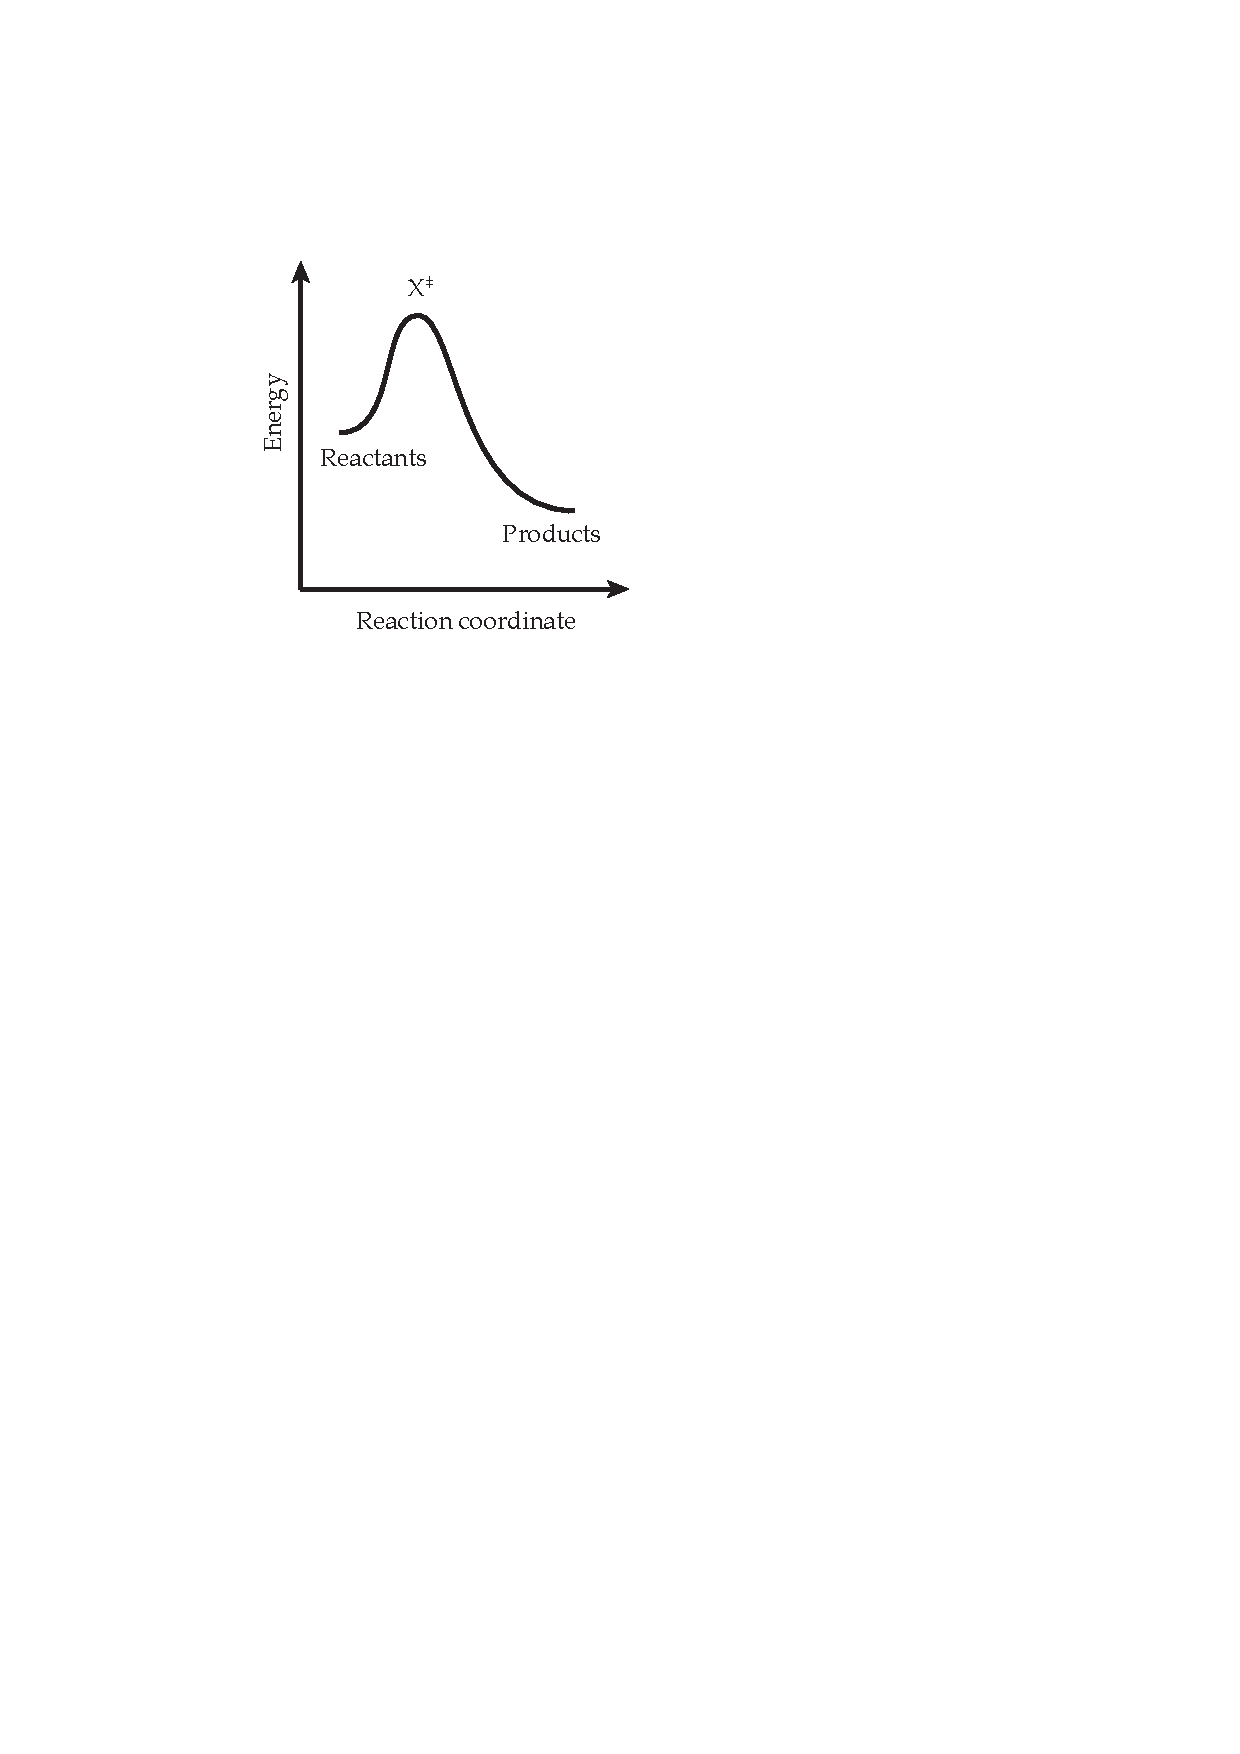
\includegraphics{TST-2D-PES}
  \caption{2-D representation}
  \label{fig:sub1}
\end{subfigure}%
\begin{subfigure}[t]{.5\textwidth}
  \centering
  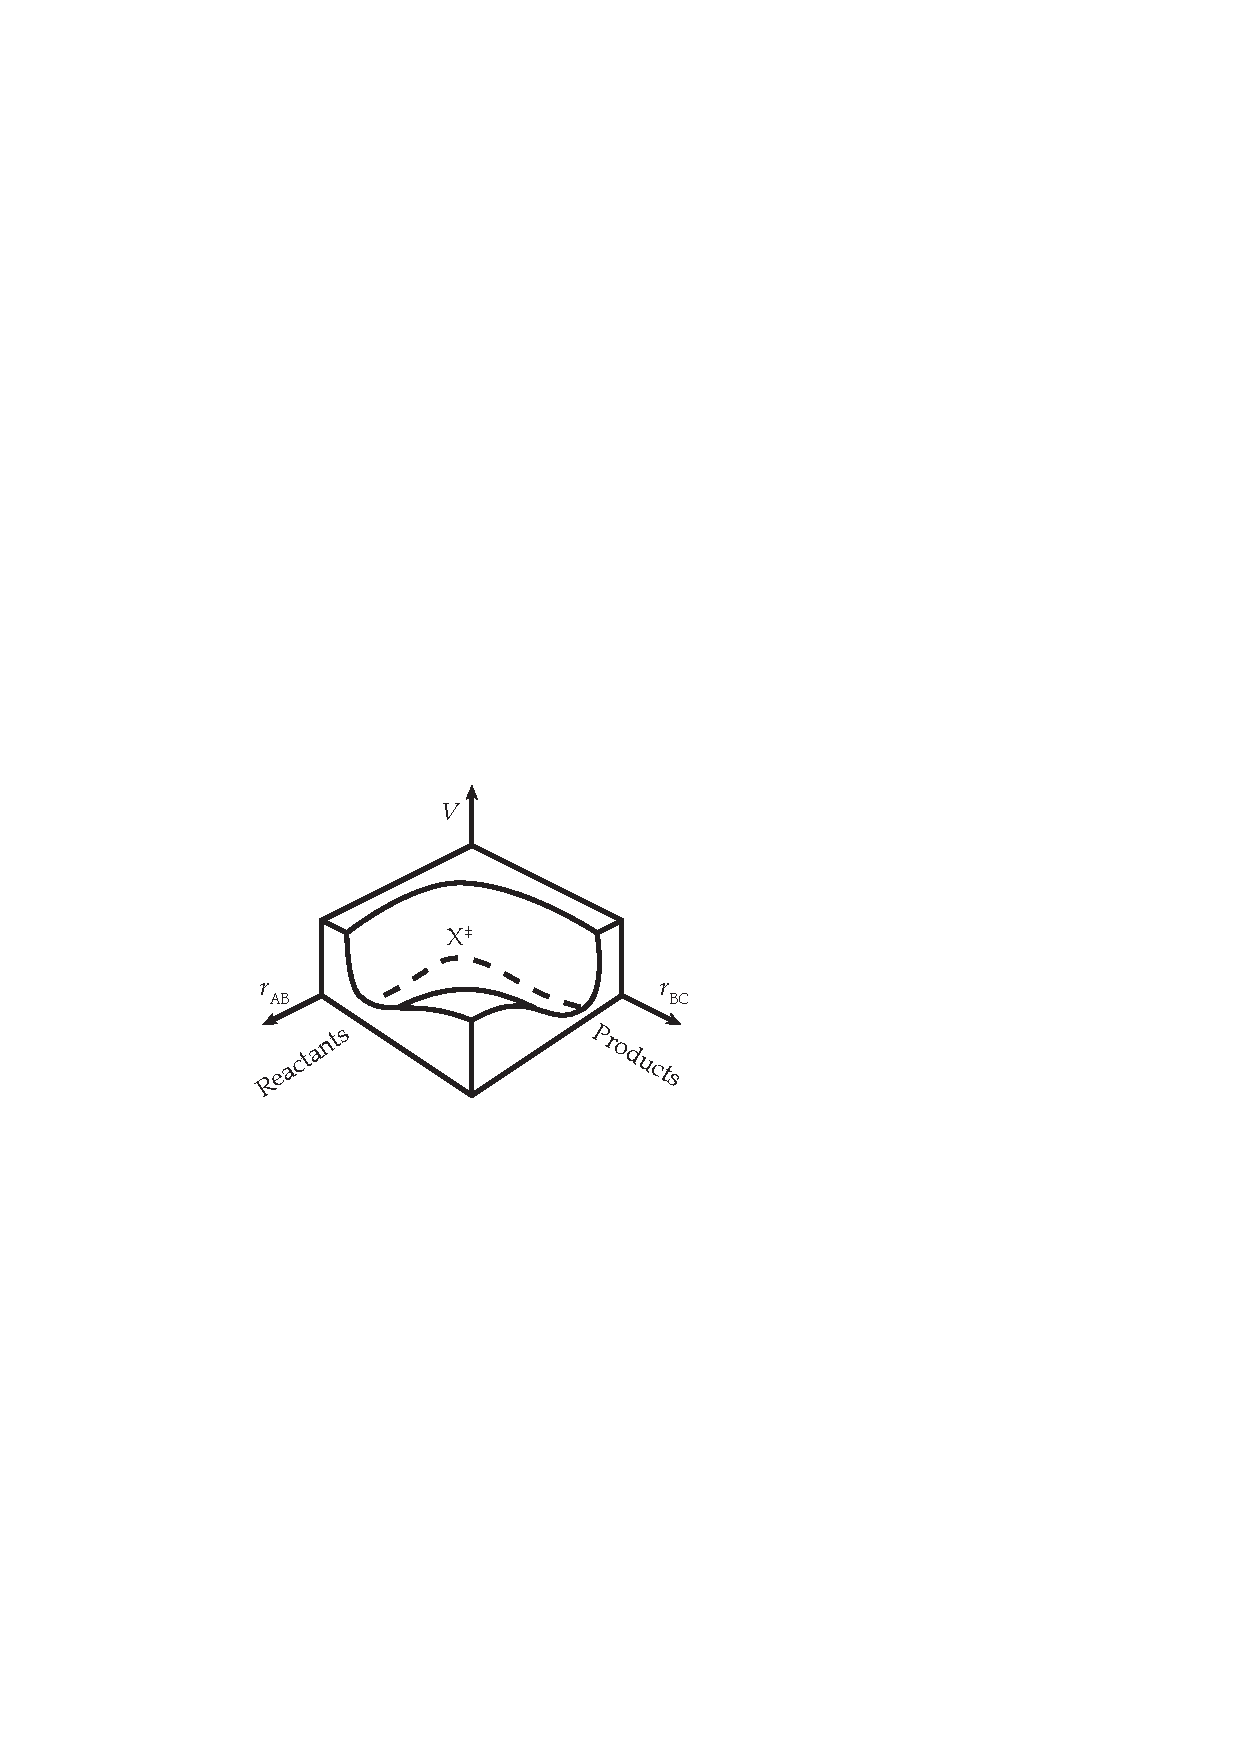
\includegraphics{TST-3D-PES}
  \caption{3-D representation}
  \label{fig:sub2}
\end{subfigure}
\caption{And example of a 1 dimensional potential energy surface. The minima represent the energy of reactant and product geometries while the maximum ($X^\ddagger$) represents the energy of the activated complex, or TS.}
\label{fig:pes}
\end{figure}


\subsection{Electronic structure calculations}

One of the fundamental concepts of TST is electronic structure calculations.
These calculations involve using the coordinates of a species or a TS to estimate the energy and forces \cite{simons:2003} which are used to optimize geometries to an energy minima (in the case of species optimization) or to a first order saddle points (in the case of a TS search).
Electronic structure calculations can also determine hindered rotor potentials as described in later sections. 
Calculations can be performed using differing degrees of fidelity, otherwise know as levels of theory. 
In general, a high level of theory will result in higher fidelity calculations and more accurate results.
We aim to highlight how electronic structure calculations are performed in four broad levels of theory: force fields, Hartree-Fock (HF) / semi-empirical methods, density functional theory (DFT), and coupled cluster calculations. 

\subsubsection{Force fields}

Force fields use attractive and repulsive parameters between atoms to calculate the potential energy of a system \cite{gonzalez:2011}. 
These parameters are often obtained from higher level of theory calculations (e.g. density functional theory or coupled cluster calculations), and describe the forces based on the distance between two bonded atoms, angles between three bonded atoms, dihedrals between four bonded atoms, non-bounded electrostatic forces, and van der Waals interactions.
Two widely used force fields are the universal force field (UFF) \cite{UFF:1992} and the Merck Molecular force field (MMFF) \cite{MMFF94:1996}.
The UFF uses parameters for bonds, angles, dihedrals, inversions, electrostatic forces, and van der Waals interactions from literature sources or extrapolations to determine the energy of a complex containing any atom type.
The MMFF includes parameters for the same geometric features as the UFF, in addition to parameters for out of plane bending often resulting in higher fidelity calculations. 
Parameters for the MMFF are included for all organic atom types and were determined from 2,775 structures optimized with either HF or semi-emperical methods.
Force field calculations are known for giving rough potential energy estimates with little computational resources, and force fields will be referred to as a ``level 0'' (L0) level of theory.

\subsubsection{Hartree-Fock and semi-empirical methods}

Hartree-Fock methods are a way to approximate the quantum wave function of a molecule at a stationary state \cite{HF:1951, HF:1987} by assuming: the molecular wave function is dependant on the coordinates of each atom's nuclei and their electrons, the solution to the wave function is a linear combination of basis functions, each energy eigenvector is solved by a single Slater determinant, and Coulomb correlations of electrons and London dispersion effects are approximated using mean field theory.
%\todo{HF uses mean field theory to simplify the electron coulomb correlation,  it does not fully neglect it. It is described well on p.34 in Jensen's Introduction to Computational Chemistry book in the DFT QC books folder in Dropbox.  He uses the solar system as an analogy.  In the HF method, you would calculate Earth's orbit by considering the gravitational force from the sun (nucleus) and the average of the gravitational forces from all the other planets}
From these assumptions, Fock matrices are constructed to approximate the energy operator of each orbital of the molecular system using basis functions.

Semi-empirical methods are based on HF methods, but use additional parameters determined from empirical data \cite{SEMethods:2014}. 
By using these empirical data, additional electron correlations and dispersion effects can be accounted for, making these methods slightly more accurate than most HF methods.
HF and semi-empirical methods will be defined as a ``level 1'' (L1) level of theory throughout this paper. 

\subsubsection{Density functional theory}

DFT approximates the wave function using functionals describing the spatial density of electrons in a molecular system, and can be used to approximate the potential acting on electrons \cite{DFT:1964,dft:1994}.
Once the wave function has been approximated, energy and forces can be calculated and minimized to obtain optimized geometries.
Depending on the functionals used, different solutions of the wave function can be approximated, making this method highly dependant on both exchange and correlation interactions. 
In general it is more accurate than HF and semi-empirical methods.
DFT will be defined as a ``level 2'' (L2) level of theory throughout this paper.

\subsubsection{Coupled cluster}

Coupled cluster (CC) methods are another way to describe many-body systems \cite{CC:2002}, and are based on HF molecular orbital methods but instead constructs a mutli-electron wave function to account for electron interactions missing from HF.
These methods offer more accurate treatment of electronic correlation than both HF and DFT, often resulting high fidelity calculations. 
CC methods are often the most accurate form of calculations that can be performed. However, their increase in accuracy is met by an increase in computational cost.
CC methods include single (S), double (D), triple (T), quadruple (Q) excitations and excitation combinations as well.
One of the more common CC methods is CCSD(T) (the single, double, and pertubative triple excitation) and it was often seen as the ``gold standard'' in that it offers a good balance between accuracy and cost.
The accuracy of CC is highly dependent on the basis set size, and by choosing combinations of different excitation levels, cluster operators are created that can approximate the wave function based on a reference wave function.
Because of the computational cost, these calculations are often reserved for single point (SP) calculations rather than for geometry optimizations.
CC calculations will be defined as a ``level 3'' (L3) level of theory.

%\todo{can have higher order excitations as well (beyond Q),  I would mention CCSD(T) method here which is Single, Double, Pertubative Triple.  It is the most popular methods and known as the 'gold standard' and offers the best accuracy to cost. Going beyond (T) doesn't add much accuracy unless it's a multireference molecule.  You might also want to mention that CC method accuracy is highly dependent on basis set size.  Need to extrapolate to complete basis set limit (CBS) or use F12 with big basis sets}


\subsection{Conformer Analysis}

In order to ensure that TST calculations are accurate, the lowest energy conformers for species and TSs must be identified.
This process is trivial for simple species or TS geometries, but becomes increasingly complex with many rotatable dihedrals, invertable double bonds, and invertable chiral centers. 
Geometries that contain $\alpha$ number of rotatable dihedrals scanned in $\theta$ degree increments, with $\beta$ number of invertable double bonds and $\gamma$ number of invertable chiral centers will result in $N$ number of possible conformers given by: 
\begin{equation}
    N = \Big(\frac{360^\circ}{\theta}\Big)^{\alpha} \cdot 2^{\beta} \cdot 2^{\gamma}
    \label{eq:confs}
\end{equation}

The evaluation of all $N$ conformers will result in a systematic search that identifies the global minima but requires large amounts of computational resources, pushing researchers have towards stochastic methods \cite{Ebejer:2012}, such as Monte Carlo methods or Genetic Algorithms to identify low energy conformers. 
These stochastic methods involve a guided exploration of a smaller portion of the conformational space.
Ideally, this results in the lowest energy, conformer but that is not always the case given the number of local minima present in conformational space.


\subsection{Canonical Partition Function}

TST makes a series of assumptions in order to arrive at kinetic parameters. 
First, it is assumed that both reactants and TS are in a quasi-equilibrium state \cite{QSS:2017}.
Additionally, it is assumed that the rate limiting step is the transition from the TS to the products. 
From these assumptions, a modified form of the Eyring equation (equation \ref{eyring:1}) is used to relate the thermodynamic properties of the TS and reactants to the elementary rate of reaction \cite{eyring:1935}.

\begin{equation}
    k(T) = \kappa \frac{k T}{h} \exp{\frac{-\Delta G^\ddagger}{RT}}
    \label{eyring:1}
\end{equation}

In equation \ref{eyring:1}, $k$ is the Boltzmann constant, $T$ is the temperature, $h$ is Plank's constant, $\Delta G^\ddagger$ is the change in Gibb's energy between the TS and the reactants,  $R$ is the gas law constant, and $\kappa$ is the correction faction for quantum tunneling described by equation \ref{tunneling}:

\begin{equation}
    \kappa = e^{\frac{V}{kT}} \int^{\infty}_{E_0} \frac{K e^{\frac{-E}{kT}}}{kT} dE
    \label{tunneling}
\end{equation}

Tunneling is the probability a particle will tunnel through a barrier without having to overcome that barrier \cite{RUBAKOV:1984}.
In this case, reactants will form products even if the barrier height is large and system energy is low. 
The correction factor for tunneling can be calculated though equation \ref{tunneling}, where $V$ is the barrier height, $E$ is energy, and $K$ is the transmission probability for tunneling.
$K$ is dependant on the energy, the shape of the barrier, and the effective mass of the system, described in detail by Brown \cite{Brown:1981}.
Equation \ref{eyring:2} can be obtained, from \ref{eyring:1}, though statistical thermodynamics.

\begin{equation}
    k(T) = \kappa \frac{k T}{h} \frac{Q^\ddagger}{\prod^{n}_{i} Q_i} \exp{\frac{-\Delta E^{\ddagger}_{0}}{k T}}
    \label{eyring:2}
\end{equation}

$Q^\ddagger$ represents the canonical partition function of the TS, $\prod^n_i Q_i$ is the product of the partition functions of $n$ number of reactants, $\Delta E^{\ddagger}_0$ is the activation energy for this reaction.
These equations can only be used if the partition functions of the reactants, products, and TS are known. 

The rigid rotor harmonic oscillator approximation is frequently used to calculate the overall partition function.
This approximation treats the the bond as a system with a resting equilibrium distance and a force constant that restores changes in bond length to its equilibrium distance.
The total partition function, $Q_{tot}$, is the product of the translational ($Q_{trans}$), rotational ($Q_{rot}$), vibrational ($Q_{vib}$), and electronic ($Q_{elec}$) partition functions of a molecule. 

\begin{equation}
    Q_{tot} = Q_{trans} Q_{rot} Q_{vib} Q_{elec}
    \label{qtot}
\end{equation}

\begin{equation}
    Q_{trans} = V \bigg( \frac{2 \pi M k_B T}{h^2} \bigg)^{\frac{3}{2}}
    \label{qtrans}
\end{equation}

\begin{equation}
    Q_{rot} = \frac{\sqrt{\pi}}{\sigma_{ext}} \bigg( \frac{8 \pi I_m k_B T}{h^2} \bigg)^{\frac{3}{2}} ; I_m = I_x I_y I_z
    \label{qrot}
\end{equation}

\begin{equation}
    Q_{vib} = \prod_i \bigg(1- \exp{\frac{-h \nu_i}{k_B T}} \bigg)^{-1}
    \label{qvib}
\end{equation}

\begin{equation}
    Q_{elec} = \sum_i g_i \exp{\frac{ -\epsilon_{ele,i}}{k_B T}} \approx g_0
    \label{qelec}
\end{equation}

All parameters, aside from constants and temperature, are unique to a specific molecule.
The translational partition function is related to the volume  $V = k_B T/p$, and the  weight of the molecule.
The rotational partition function is related to the moments of inertia, $I_x$, $I_y$ and $I_z$, and the molecular symmetry, $\sigma_{ext}$ -- the determination of which is discussed in subsequent sections.
The vibrational partition function is related to the vibrational frequencies, $\nu_i$, of each vibrational mode in the molecule.
Finally, the electronic partition function is the sum of states over electronic energies, $\epsilon_{ele,i}$, with degeneracies, $g_i$. 
It is often assumed the lowest energy state is the only one available (valid unless the first excited energy level is unusually low) so $Q_{elec}=g_0$.

\subsubsection{Hindered rotors}
An internal rotor is a non-terminal single bond with rotatable tops on either end. 
In the harmonic oscillation (H.O.) approximation, torsional rocking about this bond is modelled as harmonic motion within a potential energy well, following a potential curve described by equation \ref{eq:HO}, where $V_{H.O.}$ is the potential energy, $k$ is the spring constant, and $\Theta$ is the degree of rotation of the torsion.
\begin{equation}
    V_{H.O.} = \frac{1}{2} k \Theta^2
    \label{eq:HO}
\end{equation}
%although the true potential energy can often be more irregular than a harmonic one. 
At low temperatures the H.O. approximation holds true. However, at very high temperatures, the compound has enough energy that the hindrance between wells is negligible and so rotors can be represented as a free rotors. 
Hindered rotors (H.R.) occur at intermediate temperatures where the compound has enough energy to rotate out of one conformer and into another, but not enough energy for hindrance to be negligible.

The calculation of the partition function can be further expanded by using the 1-D hindered rotor approximation \cite{pfaendtner:2007}.
In this approximation, each side of a four atom dihedral is considered a separable rotatable top.
Starting from a minimum energy structure, the potential energy is determined using electronic structure calculations as one top is rotated over \ang{360}. 
This potential energy curve is fitted to a Fourier series described in equation \ref{eq:HR}:

\begin{equation}
    V(\Theta_j)_{H.R.} = \sum^{n}_{k=1} \Big[ a_k (1 - \cos{k \Theta_j}) + b_k \sin{k \Theta_j} \Big]
    \label{eq:HR}
\end{equation}

Where $V$ is the potential energy as a function of the rotation of the torsion of interest $\Theta$, $n$ is the number of scanned points (e.g. if the scan was performed over \ang{10} intervals, $n$ would be 36), and $a_k$ and $b_k$ are fitted parameters.
It is noted that the above equations are used to represent 1-D hindered rotors which are completely separable.
Treatment of coupled hindered rotors (e.g. 2-D and 3-D) is not discussed in this review, but is discussed Fern\'andez-Ramos' paper on the treatment of 2-D rotors \cite{fernandez:2013}.


\subsubsection{Symmetry number}

A symmetry number is the number of different but equivalent arrangements of a molecule or a TS geometry \cite{FernandezRamos:2007}.
Accurately determining the symmetry number of species and TS geometries is imperative to calculating thermodynamic and kinetic parameters, the symmetry number is included in the rate expression.
For a majority of cases, rotational symmetry numbers are adequate when describing the overall external symmetry number of stable species and can be calculated using equation \ref{eq:symm}.

\begin{equation}
    \label{eq:symm}
    \sigma_{ext} \approx \sigma_{rot} = \frac{m!}{n_d}
\end{equation}

In the above equation, $\sigma$ is the rotational symmetry number, $m!$ is the number of permutation of $m$ equivalent atoms, and $n_d$ is the number of distinguishable configurations or orientations of molecules that cannot be mapped onto another configuration by rotation.
For example, when considering ammonia (\ce{NH3}), there are three equivalent hydrogen atoms and two distinguishable configurations of those atoms resulting in a rotational symmetry number of three.
Rotational symmetry numbers of TS geometries can be taken as the product of the rotational symmetry numbers of the stable species, shown in equation \ref{eq:symm_ts}, where $n$ is the number of reactants in a reaction and $\sigma_{rot,i}$ is the rotational symmetry number for the $i$th reactant.

\begin{equation}
    \sigma_{TS,rot} = \prod^n_{i=1}\sigma_{rot,i}
    \label{eq:symm_ts}
\end{equation}

For TSs of bimolecular reactions between identical species, the rotational symmetry number is not sufficient when determining the overall symmetry number of a geometry.
In this case, it is better to use the rotational translational symmetry number, $\sigma_{r-t}$, which takes into account translational symmetry.
For example, assume the reaction \ce{A_i + A_j -> Products} has a TS geometry, $R$, where $i$ and $j$ are labels to distinguish between identical \ce{A} species.
In this case, the rotational symmetry number would be $\sigma_{rot,R} = \sigma_{rot,A}^2$ but this does not account for the translation of identical molecule (e.g. \ce{A_i + A_j} in 3D space compared to \ce{A_j + A_i}), so the rotational translational symmetry number would be $\sigma_{rot,R} = 2\sigma_{rot,A}^2$. 
The factor of two accounts for the translational exchange of positions of \ce{A_i} and \ce{A_j} via translation.
Additional explanations of symmetry numbers are described by Fern\'andez-Ramos and co-workers \cite{FernandezRamos:2007}.


%%%%%%%%%%%%%%%%%%%%%%%%%%%%%%%%%%%%%%%%%%%%%%%%%%%%%%%%%%%%%%%%%%%%%%%%%%%%%%%%%%%%
%%%%%%%%%%%%%%%%%%%%%%%%%%%%%%%%%%%%%%%%%%%%%%%%%%%%%%%%%%%%%%%%%%%%%%%%%%%%%%%%%%%%
%%%%%%%%%%%%%%%%%%%%%%%%%%%%%%%%%%%%%%%%%%%%%%%%%%%%%%%%%%%%%%%%%%%%%%%%%%%%%%%%%%%%


\section{Automated transition state theory code bases}

This section of the review introduces existing code bases that can perform automated TST calculations, highlights and compares their key features and their methodology, and briefly discusses their test sets.

%%%%%%%%%%%%%%%%%%%%%%%%%%%%%%%%%%%%%%%%%%%%%%%%%%%%%%%%%%%%%%%%%%%%%%%%%%%%%%%%%%%%
%%%%%%%%%%%%%%%%%%%%%%%%%%%%%%%%%%%%%%%%%%%%%%%%%%%%%%%%%%%%%%%%%%%%%%%%%%%%%%%%%%%%
%%%%%%%%%%%%%%%%%%                                                %%%%%%%%%%%%%%%%%%
%%%%%%%%%%%%%%%%%%                     AutoTST                    %%%%%%%%%%%%%%%%%%
%%%%%%%%%%%%%%%%%%                                                %%%%%%%%%%%%%%%%%%
%%%%%%%%%%%%%%%%%%%%%%%%%%%%%%%%%%%%%%%%%%%%%%%%%%%%%%%%%%%%%%%%%%%%%%%%%%%%%%%%%%%%
%%%%%%%%%%%%%%%%%%%%%%%%%%%%%%%%%%%%%%%%%%%%%%%%%%%%%%%%%%%%%%%%%%%%%%%%%%%%%%%%%%%%

\subsection{AutoTST (2016)}

AutoTST, developed by Bhoorasingh et al., is one of the first automated TST tools designed to work for gas phase reactions in combustion settings \cite{bhoorasingh:2017}.
AutoTST began as a module included within the Reaction Mechanism Generator (RMG) package which uses RMG reaction objects to perform calculations and is freely available under the MIT license. 
The overall workflow for AutoTST is shown in figure \ref{fig:autotst_overview}.

This tool does not require users to provide geometry input files or guesses for key reaction coordinates contrary to required inputs of most quantum chemistry packages.
A user manually matches an RMG reaction object to one of three reaction families (hydrogen abstraction, intramolecular hydrogen migration, and radical addition to multiple bond): from there AutoTST calculates kinetics. 

\begin{figure}[h!]
    \centering
    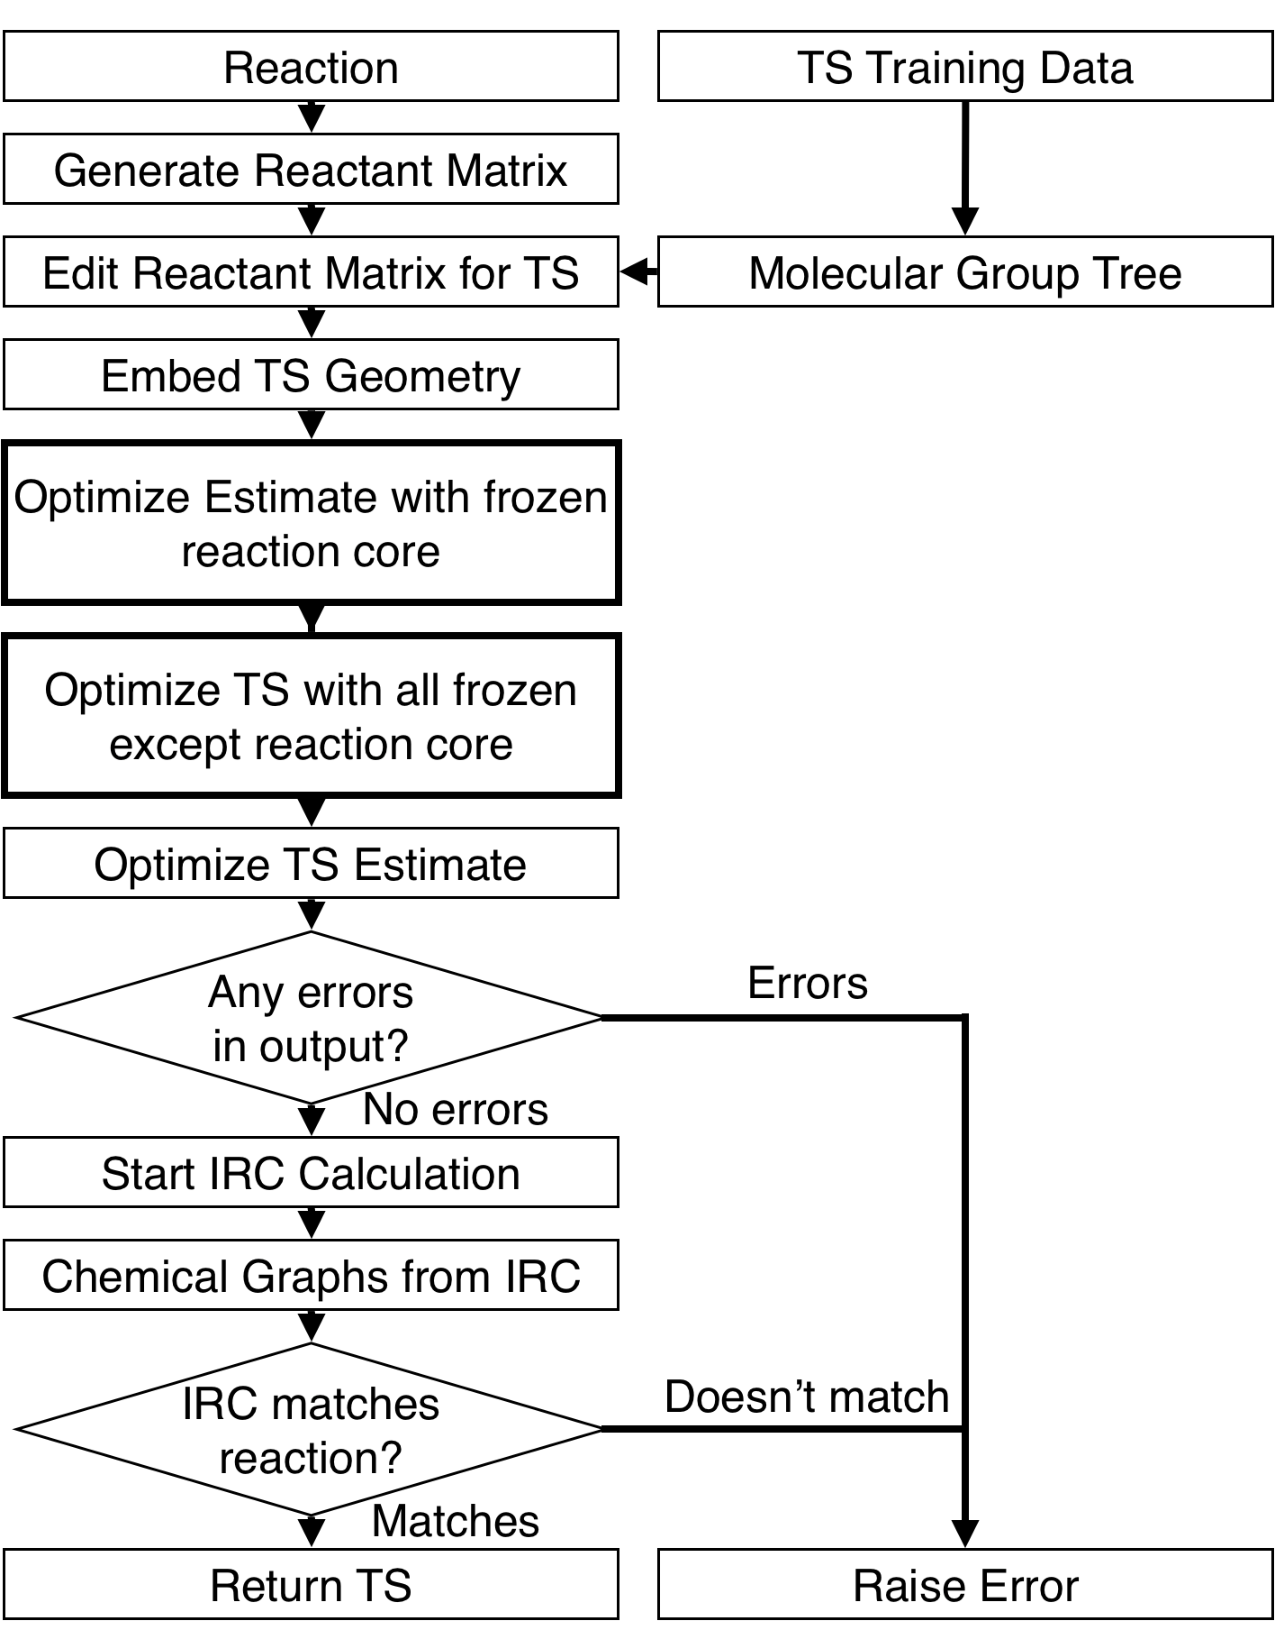
\includegraphics[width=0.75\textwidth]{autotst_overview}
    \caption{A flow chart describing the workflow of AutoTST, modified from \cite{bhoorasingh:2017}. Training data are used to estimate the TS geometry. This geometry is then optimized using a set of partial optimizations and validated using IRC calculations.}
    \label{fig:autotst-overview}
\end{figure}

Predictions of distances between reacting atoms are made based on a hierarchical decision tree corresponding to a reaction family.
The reaction is matched to a node on the tree based upon functional groups near the reacting atoms. This node specifies the distances between reacting atoms.
A depiction of a tree is given in figure \ref{fig:autotst_tree}.

\begin{figure}[h!]
    \centering
    
\includegraphics[width=0.5\textwidth]{autotst_tree}
    \caption{An example of a decision tree used in AutoTST. Reacting atoms are matched to a node on the tree to provide key distances in the reaction center. If no exact match exists or data does not exist for an exact match, a general match on a higher node will be used.}
    \label{fig:autotst_tree}
\end{figure}

With these key distances, AutoTST then employees RDKit \cite{RDKit:2018} to generate three-dimensional geometries of reactant, product, and TS geometries.
Reactant and product geometries are created using RDKit's built-in embed feature at an L0 level of theory. 
A bounds matrix describing upper and lower allowable distances between atoms is generated for TS geometries and the distances between reacting atoms are set according to key distances.
This matrix is used to generate a 3D geometry guess of the TS.
The guess of the TS geometry then goes through a series of optimizations at a L2 level of theory: (1) a loose geometry relaxation with distances in the reaction center frozen; (2) a constrained saddle point search with the the reaction center fixed; and (3) a tight overall saddle search of the TS geometry without constraints.
If AutoTST converges on a final TS, it validates the TS via intrinsic reaction coordinate (IRC) calculations \cite{Fukui:1970} and cross checks these results with the input reactants and products.
Once TS, reactant, and product geometries are known and validated, Arkane \cite{gao:2016}, a canonical calculator included in RMG, is used to arrive at modified Arrhenius parameters.

To test this work flow, Bhoorasingh and coworkers attempted calculations for 1117 reactions present in a model for the combustion of butanol and four of its isomers \cite{Sarathy:2012}.
Of these reactions, 885 were hydrogen abstraction reactions, 78 were intramolecular hydrogen migration reactions, and 184 were radical addition to multiple bond reactions. 
For each of these reaction families, AutoTST had success rates of approximately 70\%,summarized in table \ref{table:ModelRxns}.

\begin{table}[h!]
\label{t:atst_r}
\small
\caption{\label{table:ModelRxns} Number of reactions for each family contained in the combustion model, and success of the AutoTST algorithm.}
\centering
\begin{tabular*}{\linewidth}{@{\extracolsep{\fill}}lccc}
\hline\rule{0pt}{2.6ex}%
Reaction Family & Number of  & Kinetics successfully & Percentage \\
  & Reactions  & calculated & calculated\\
\hline\rule{0pt}{2.6ex}%
Hydrogen abstraction & 855 & 598 & 70\% \\
Intramolecular hydrogen migration & 78 & 52 & 67\% \\
Radical addition to multiple bond & 184 & 131 & 71\% \\
\hline\rule{0pt}{2.6ex}%
Total & 1117 & 781 & 70\%\\
\hline
\end{tabular*}
\end{table}

A majority of AutoTST calculated kinetics agreed well with kinetics reported in the original model and estimates by RMG, however some had large disagreements with published kinetics. 
Based on error analysis against benchmark calculations, Bhoorasingh and co-workers commented that AutoTST's workflow would benefit from a detailed conformational analysis and hindered rotor treatment. 

%%%%%%%%%%%%%%%%%%%%%%%%%%%%%%%%%%%%%%%%%%%%%%%%%%%%%%%%%%%%%%%%%%%%%%%%%%%%%%%%%%%%
%%%%%%%%%%%%%%%%%%%%%%%%%%%%%%%%%%%%%%%%%%%%%%%%%%%%%%%%%%%%%%%%%%%%%%%%%%%%%%%%%%%%
%%%%%%%%%%%%%%%%%%                                                %%%%%%%%%%%%%%%%%%
%%%%%%%%%%%%%%%%%%                     AutoTS                     %%%%%%%%%%%%%%%%%%
%%%%%%%%%%%%%%%%%%                                                %%%%%%%%%%%%%%%%%%
%%%%%%%%%%%%%%%%%%%%%%%%%%%%%%%%%%%%%%%%%%%%%%%%%%%%%%%%%%%%%%%%%%%%%%%%%%%%%%%%%%%%
%%%%%%%%%%%%%%%%%%%%%%%%%%%%%%%%%%%%%%%%%%%%%%%%%%%%%%%%%%%%%%%%%%%%%%%%%%%%%%%%%%%%

\subsection{AutoTS (2017)}

AutoTS is a framework introduced by Jacobson et al. from Schrodinger Inc. \cite{jacobson:2017}. 
This workflow is included in Jaguar version 9.7 \cite{Jaguar:2013}, a commercial quantum chemistry package provided by Schrodinger Inc., shown in figure \ref{fig:autots_workflow}.
AutoTS and Jaguar are available through proprietary license for purchase.

This tool requires users to provide geometries of the reactants and products in 3D Cartesian coordinates, assumed to be at a stable energy minima.
AutoTS determines reacting bonds and atom correspondence through an iterative bond deletion method by systematically breaking a bonds, generating canonicalized SMILES strings for the modified reactant and product complexes, and comparing said strings.
The algorithm will first start by deleting zero bonds and if the complexes are not identical, it will break one bond at a time.
If the complexes are not identical after deleting one bond at a time, the algorithm will break two at a time by systematically looping through all possible combinations of bonds.
This process will continue searching up to a maximum number of broken bonds, the default being four bonds.
Once active bonds are identified, input geometries of reactant and product complexes can be used to create the TS guess.

AutoTS can generate TS guesses by linear searches or by templating. 
A linear search involves aligning reactant and product geometries by positioning the reactant and product molecules at opposite corners of a cube with a size large enough to allow for molecules to not overlap.
This geometry is then rotated until the inertial tensor is diagonalized to create a standard reproducible geometry.
The format TS guess is created by calculating energies along a linear distance coordinate path connecting the reactants and products, using an L2 level of theory.
Interpolation along cubic splines is used to identify the energy maximum geometry to be used as the starting TS guess.

Templating can create guesses by using ``templates''  from previously optimized TS geometries which are contained in an auxiliary file containing geometries for successfully calculated TSs and string representations of the corresponding reactions.
Subgroup complexes are then generated of the $i$th order by including the ($i-1$)th neighboring atoms in the reaction center. 
If a match exists in the auxiliary file, the matching atoms are set to the corresponding atoms in the previously run TS to generate a new TS guess and  then optimized using quadratic synchronous transit and a quasi-Newton eigenvector at a L2 level of theory.

TSs are verified through two processes: ``vetting'' and ``connecting''. 
Vetting assesses if the TS meets three criteria: (1) there is exactly one imaginary frequency; (2) the TS geometry has at least one activate bond at an intermediate distance; and (3) the translational mode corresponding to the imaginary frequency contains motion along an active bond.
If vetting is successful, the TS complex is connected by a modified three-point IRC calculation to identify only reactant, TS, and product geometries. 
A TS is validated if connected to the input reactant and product geometries.
Although AutoTS has a robust method to find TSs, it does not return kinetic parameters, only thermodynamic parameters for reactant, product, and TS geometries.

\begin{figure}[h!]
\centering
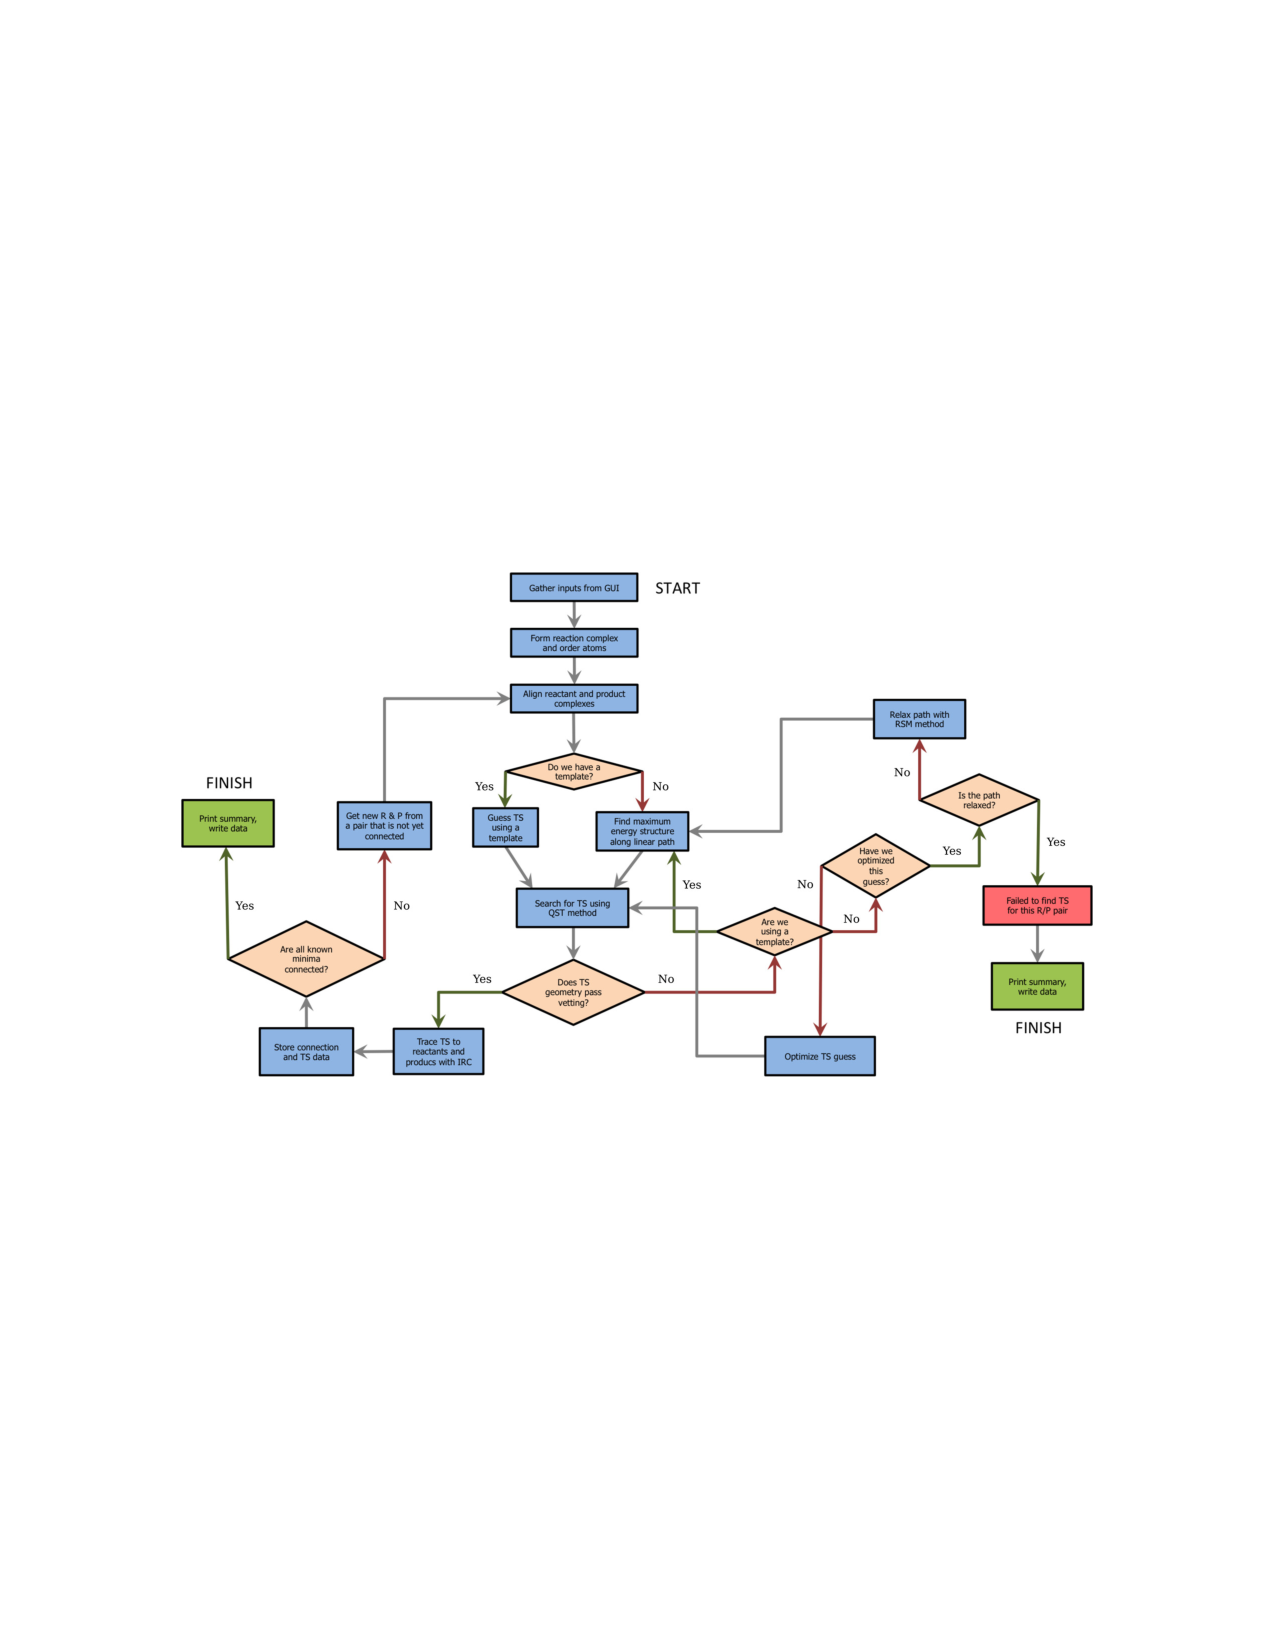
\includegraphics[width=\textwidth]{autots_workflow}
\caption{A flow diagram of AutoTS taken from \cite{jacobson:2017}. Input geometries are read and used generate TS guesses using templates or from linear interpolation. Fail-safes are in place to ensure all options are exhausted when finding the correct TS geometry.}
\label{fig:autots_workflow}
\end{figure}

To test the efficacy of AutoTS, Jacobson and coworkers used test sets for four reaction families: Michael addition, carbene insertion, hydrogen abstraction, and Diels-Alder.
AutoTS has shown great efficacy in these test cases, although the authors do highlight avenues of improvement necessary in AutoTS.
From the version of AutoTS published, the authors wished to add support of reactions that do not involve forming or breaking covalent bonds, reactions with spectator molecules, reactions involving transition metals, reactions with cage-like geometries, sterocenters of reacting atoms, conformational analysis (this version of AutoTS currently uses only the input conformation of reactants and products to generate TS geometries), and very large molecules (300+ atoms).


%%%%%%%%%%%%%%%%%%%%%%%%%%%%%%%%%%%%%%%%%%%%%%%%%%%%%%%%%%%%%%%%%%%%%%%%%%%%%%%%%%%%
%%%%%%%%%%%%%%%%%%%%%%%%%%%%%%%%%%%%%%%%%%%%%%%%%%%%%%%%%%%%%%%%%%%%%%%%%%%%%%%%%%%%
%%%%%%%%%%%%%%%%%%                                                %%%%%%%%%%%%%%%%%%
%%%%%%%%%%%%%%%%%%                     GENESYS                    %%%%%%%%%%%%%%%%%%
%%%%%%%%%%%%%%%%%%                                                %%%%%%%%%%%%%%%%%%
%%%%%%%%%%%%%%%%%%%%%%%%%%%%%%%%%%%%%%%%%%%%%%%%%%%%%%%%%%%%%%%%%%%%%%%%%%%%%%%%%%%%
%%%%%%%%%%%%%%%%%%%%%%%%%%%%%%%%%%%%%%%%%%%%%%%%%%%%%%%%%%%%%%%%%%%%%%%%%%%%%%%%%%%%

\subsection{Genesys (2018)}

An automated TST calculator was recently added to Genesys, a reaction mechanism generator software developed by Vandewiele and co-workers at Ghent University \cite{VANDEVIJVER:2018, vandewiele:2012}. 
This tool requires users to provide a description of the reaction family, identified reacting atoms, and quantum chemistry settings.
Genesys is available through proprietary license.
%A brief overview Genesys' work flow is given in figure \ref{fig:genesys_workflow}.

Reactant and product geometries are created by embedding using a L0 level of theory, followed by a rough geometry minimization at an L1 level of theory and an exhaustive conformer analysis at a user defined level of theory (often at L1 or L2 level of theory).
Low energy conformers within a specific cutoff criteria are identified and are further optimized at a user defined level of theory (often L2 level of theory).
After, the lowest energy conformer is used to perform 1-D hindered rotor scans on all rotatable bonds at a L2 level of theory.

TS complexes are generated by matching the reaction to a template to identify reacting atoms and by using key distances of the reaction center. 
Key distances are either based on previous TS searches or user specified distances.
Similar to AutoTST, 3D complexes are created by editing the bounds matrix with key distances (similar to AutoTST) and then embedded in  a 3D geometry at a L0 level of theory.
Complexes are loosely optimized to a minima while keeping the reacting atoms fixed at a L1 level of theory.
TS geometries undergo exhaustive conformer searches at a L1 or L2 level of theory calculations by relaxing geometries to a minima with a frozen reaction center.
The lowest energy conformer is optimized to a saddle point at a L2 level of theory where 1-D hindered rotor scans are performed. 
TS geometries are verified by identifying a single imaginary frequency and observing the change in bond lengths when applying Cartesian displacements of the imaginary frequency.
This is preformed in lieu of  IRC calculations to reduce computational costs.
A TS is verified if the the translational mode corresponding to the imaginary frequency contains motion along active bonds, and if these contributions are larger than that of the rest of the complex, the TS is validated. 
Validated TS, reactant, and product geometries are then used to extract Arrhenius parameters through statistical thermodynamics.

%%%%%%%%%%%%%%%%%%%%%%%%%%%%%%%%%%%%%%%%%%%%%%%%%%%%%%%%%%%%%%%%%%%%%%%%%%%%%%%%%%%%
%%%%%%%%%%%%%%%%%%%%%%%%%%%%%%%%%%%%%%%%%%%%%%%%%%%%%%%%%%%%%%%%%%%%%%%%%%%%%%%%%%%%
%%%%%%%%%%%%%%%%%%                                                %%%%%%%%%%%%%%%%%%
%%%%%%%%%%%%%%%%%%                     AARON                      %%%%%%%%%%%%%%%%%%
%%%%%%%%%%%%%%%%%%                                                %%%%%%%%%%%%%%%%%%
%%%%%%%%%%%%%%%%%%%%%%%%%%%%%%%%%%%%%%%%%%%%%%%%%%%%%%%%%%%%%%%%%%%%%%%%%%%%%%%%%%%%
%%%%%%%%%%%%%%%%%%%%%%%%%%%%%%%%%%%%%%%%%%%%%%%%%%%%%%%%%%%%%%%%%%%%%%%%%%%%%%%%%%%%

\subsection{AARON (2018)}

The open-source AARON code-base (An Automated Reaction Optimizer for New catalysts) is a Perl based software developed by Guan and co-workers to tackle automated quantum mechanic calculations for catalytic reactions involving chiral products \cite{Guan:2018}. 
AARON is freely available under the GPL-3.0 liscense.
A brief overview of the workflow is shown in figure \ref{fig:aaron_workflow}.
AARON is built on the AaronTools \cite{aarontools:2018} collection which allows users to build and modify 3D geometries by reading in \texttt{.xyz} files.

\begin{figure}
    \centering
    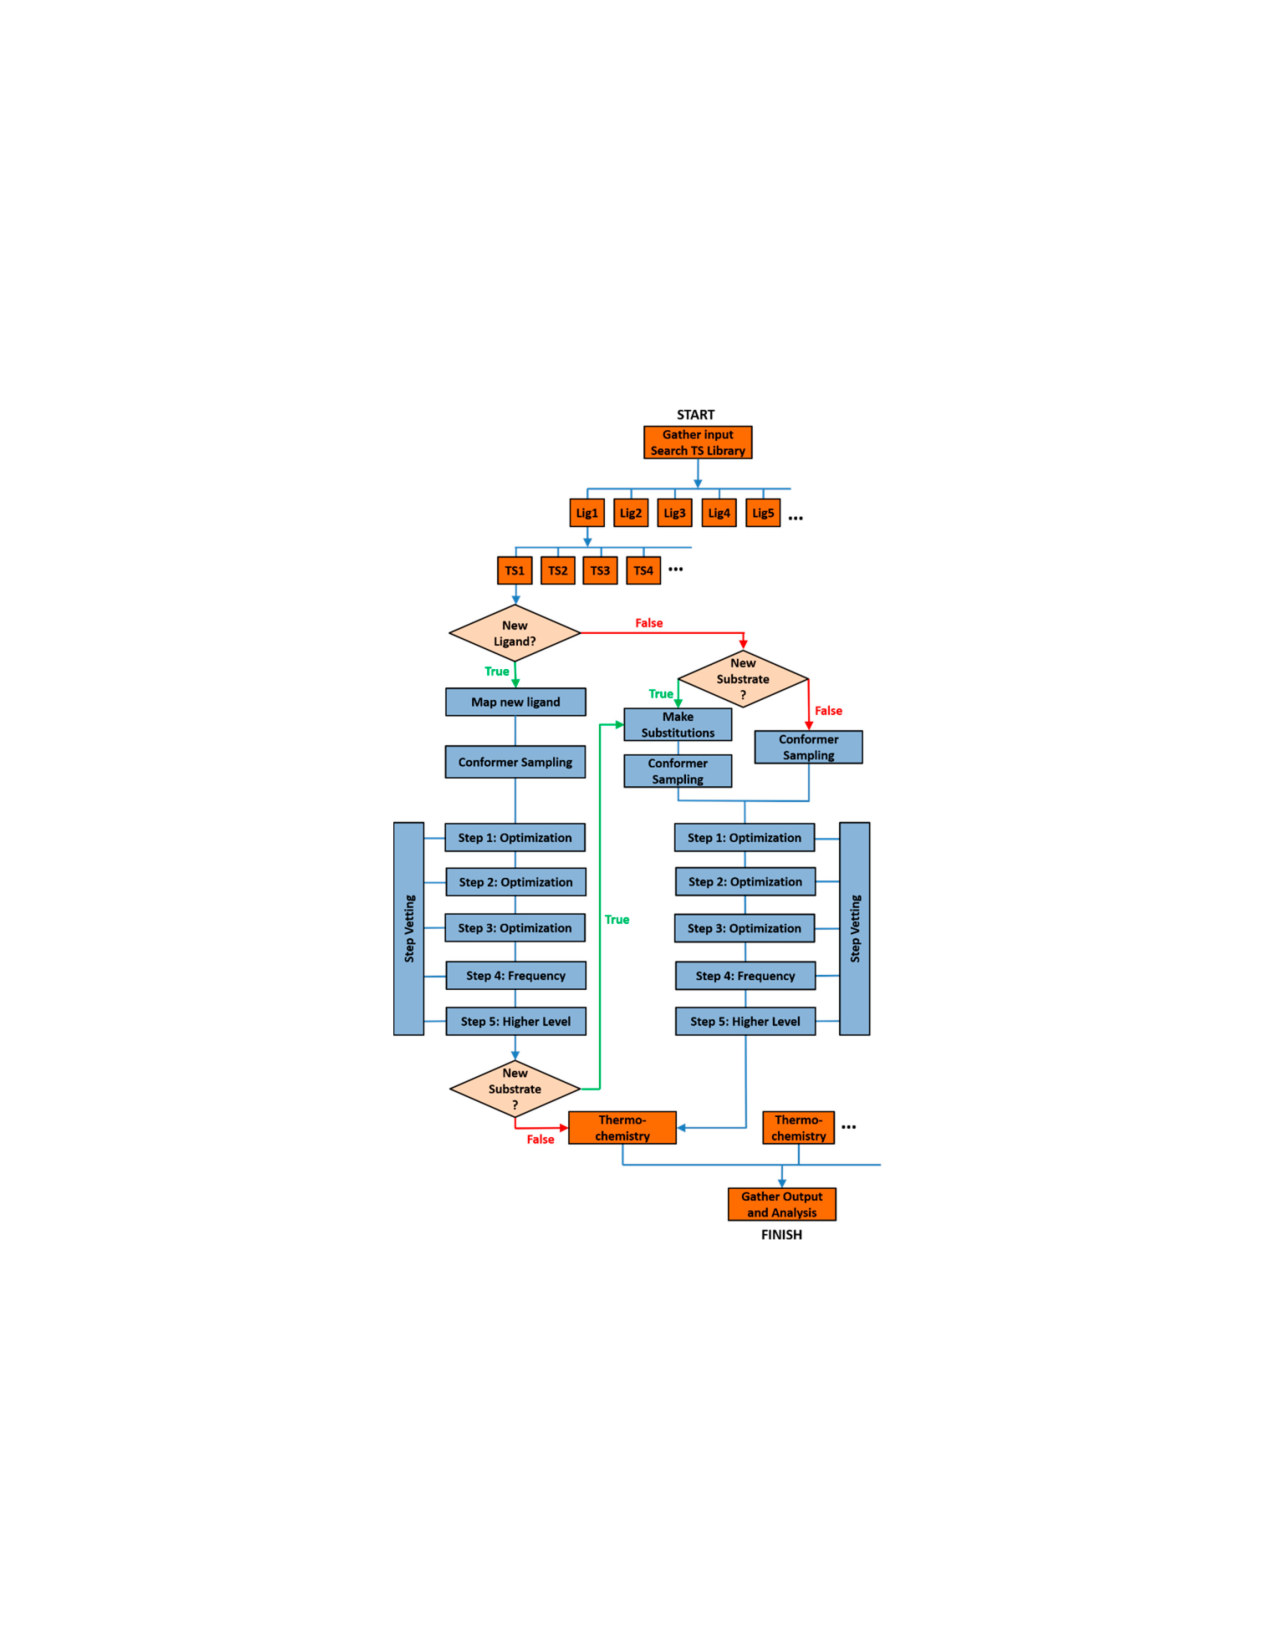
\includegraphics{aaron_workflow}
    \caption{An overview of the AARON workflow. Borrowed from \cite{Guan:2018}}
    \label{fig:aaron_workflow}
\end{figure}

AARON generates TS guesses by having users provide input files containing reactant geometries and specified reacting atoms.
AARON requires a seed library containing previously optimized geometries for a family of interest and ``templates'' the reaction similarly to AutoTS.
This involves identifying a previous geometry that closely resembles the TS of interest, setting all similar atoms to positions of the previous geometry, and replacing non-similar atoms with their correct counterparts.
The TS guesses undergo a rule based conformer analysis investigating (1) conformers for substituents  deemed ``new'' by AARON or the user, (2) torsional angles based off the symmetry of the dihedral, and (3) ``generations'' of conformers evaluated hierarchically.
For the hierarchical search, the first ``generation'' of conformers are created by rotating a single substituent and optimizing, and from that, unique conformers are identified.
These the next substituent of these unique conformers are rotated and optimized to create children for the next generation. 
If an optimized child is a duplicate of a previously identified conformer, it is not used to create future generations.
This process repeats until all substituents have been evaluated. 

Unique conformers are used in a Boltzmann-weighted sum to determine thermochemical parameters of TS complexes. 
AARON also has an error handling workflow called ``Step Vetting'' to solve problems that arise and to validate TS geometries, a diagram is given in figure \ref{fig:aaron_exception}.
This process will follow geometries through the workflow to check for common errors (e.g. breaking of non-reactive bonds, atoms clashing, and more) and attempts to correct them.

\begin{figure}
    \centering
    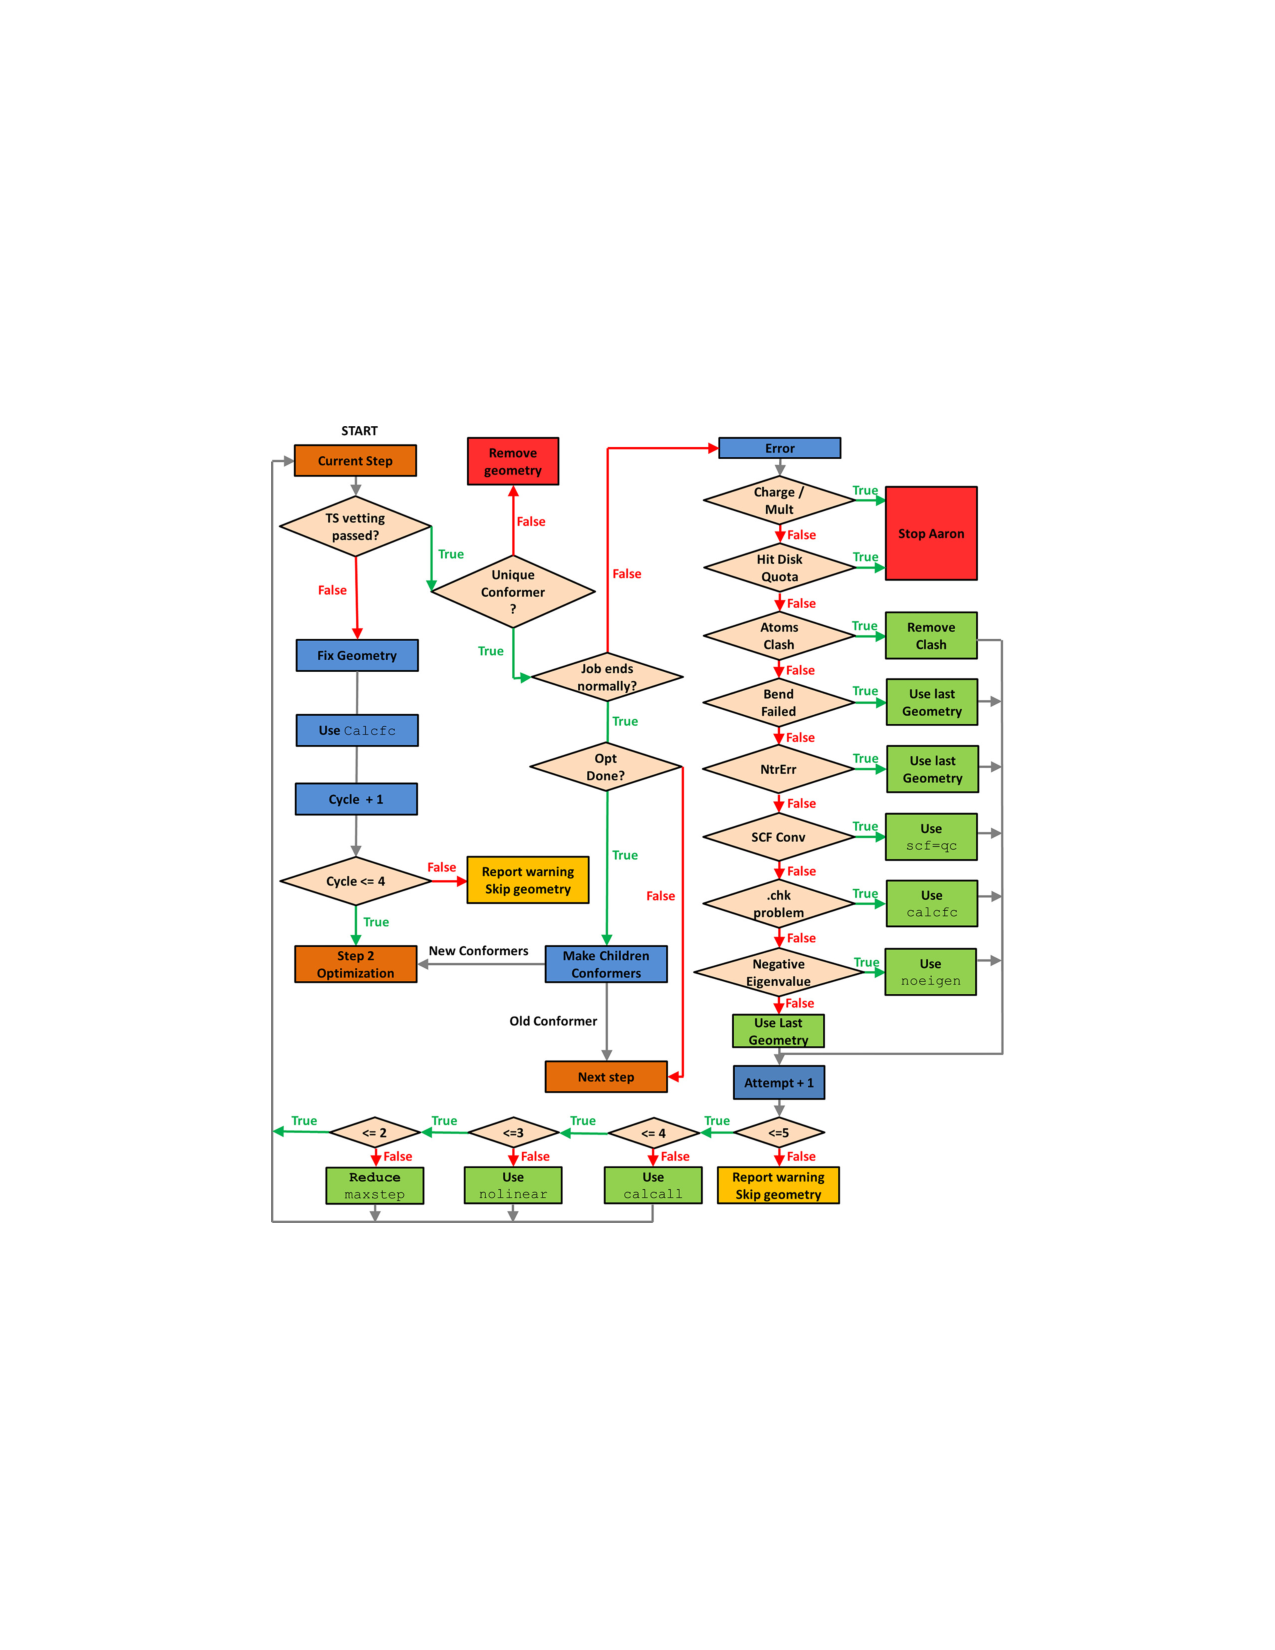
\includegraphics[width=\textwidth]{aaron_exception}
    \caption{The procedure for ``Step Vetting'' which is used in AARON to monitor jobs when searching for TS geometries.}
    \label{fig:aaron_exception}
\end{figure}

To test this workflow, the authors looked at three test sets: Pd-catalyzed Heck allenylation, Rh-catalyzed hydrogenation of enamides, and Lewis-base promoted propargylation of aromatic aldehydes.
In each test case, small template libraries were created using a published set of TS geometries with corresponding energies and used AARON to perform TS searches.
AARON was able to locate a majority of the TS geometries with good agreement in energies.

AARON is still in its early stages of development with room for improvement, specifically, creating an automated approach to create TS libraries by making use of numerous TS data generated in each run.


%%%%%%%%%%%%%%%%%%%%%%%%%%%%%%%%%%%%%%%%%%%%%%%%%%%%%%%%%%%%%%%%%%%%%%%%%%%%%%%%%%%%
%%%%%%%%%%%%%%%%%%%%%%%%%%%%%%%%%%%%%%%%%%%%%%%%%%%%%%%%%%%%%%%%%%%%%%%%%%%%%%%%%%%%
%%%%%%%%%%%%%%%%%%                                                %%%%%%%%%%%%%%%%%%
%%%%%%%%%%%%%%%%%%                    EStokTP                     %%%%%%%%%%%%%%%%%%
%%%%%%%%%%%%%%%%%%                                                %%%%%%%%%%%%%%%%%%
%%%%%%%%%%%%%%%%%%%%%%%%%%%%%%%%%%%%%%%%%%%%%%%%%%%%%%%%%%%%%%%%%%%%%%%%%%%%%%%%%%%%
%%%%%%%%%%%%%%%%%%%%%%%%%%%%%%%%%%%%%%%%%%%%%%%%%%%%%%%%%%%%%%%%%%%%%%%%%%%%%%%%%%%%


\subsection{EStokTP (2018)}


EStokTP (Electronic Structure to k(T,P)) \cite{Cavallotti:2019jctc} is an automated rate calculator by Cavallotti and Klippenstein that takes a series of input files and returns a temperature and pressure dependent rate expression and optimized electronic structures of reactants, products, and TSs.
A general program structure of EStokTP is shown in figure \ref{fig:estoktp_structure}.
EStokTP is freely available under the GPL-3.0 liscense.

Input files containing quantum methods desired, reasonable guesses for some internal coordinates, and labeled atoms describing the reaction family are used to perform calculations.
Currently, EStokTP works for four reaction families: abstraction, addition, beta scission, and isomerization. 
In the case of hydrogen abstraction inputs (shown in figure \ref{fig:estoktp_habstraction}), the user specifies the hydrogen being abstracted (\texttt{isite}), the atom bound to that hydrogen (\texttt{jsite}), and another atom connected to \texttt{jsite} (\texttt{ksite}).
In addition, a dummy atom (X) is added to the complex as a reference point for atoms in the reaction center.
Users will then specify two entry angles for reactants (\texttt{aabs1}, \texttt{aabs2}) and three dihedral angles.
%These dihedral angles are as follows: first atom of abstracting reactant, \texttt{isite}, dummy atom, \texttt{jsite}; second atom of abstracting reactant, first atom of abstracting reactant, \texttt{isite}, dummy atom; and, (if available) third atom of abstracting reactant, second atom of abstracting reactant, first atom of abstracting reactant, \texttt{isite}.
EStokTP interfaces with Gaussian \cite{Gaussian:2009} or MolPro \cite{molpro:2012} to construct the TS guess with the specified internal coordinates by positioning the reactants according to user specified internal coordinates. 
$5 + 3^n$ or $100$ conformers are generated randomly, whichever is smaller and where $n$ is the number of non-methyl dihedrals, relaxed and the highest energy conformer undergoes a series of partial optimizations to arrive at a saddle point at a L2 level of theory. 
The TS is validated  through IRC calculations, and 1-, 2-, or 3-D hindered rotor calculations are performed at a L2 level of theory.
Single point energies are calculated at a L3 level of theory.
In addition, EStokTP is also unique in that it uses a multi van der Waals well method when identifying TS geometries and kinetics.
van der Waals wells can be considered for both the reactant and product side (3TS present in abstraction reactions), just the reactant side (2TS present in addition and scission reaction), or not consider the van der Waals wells at all (1TS present in isomerization).
Reactant, product, and TS geometries are passed to EStokTP's master equation solver to obtain kinetic parameters.


\begin{figure}
    \centering
    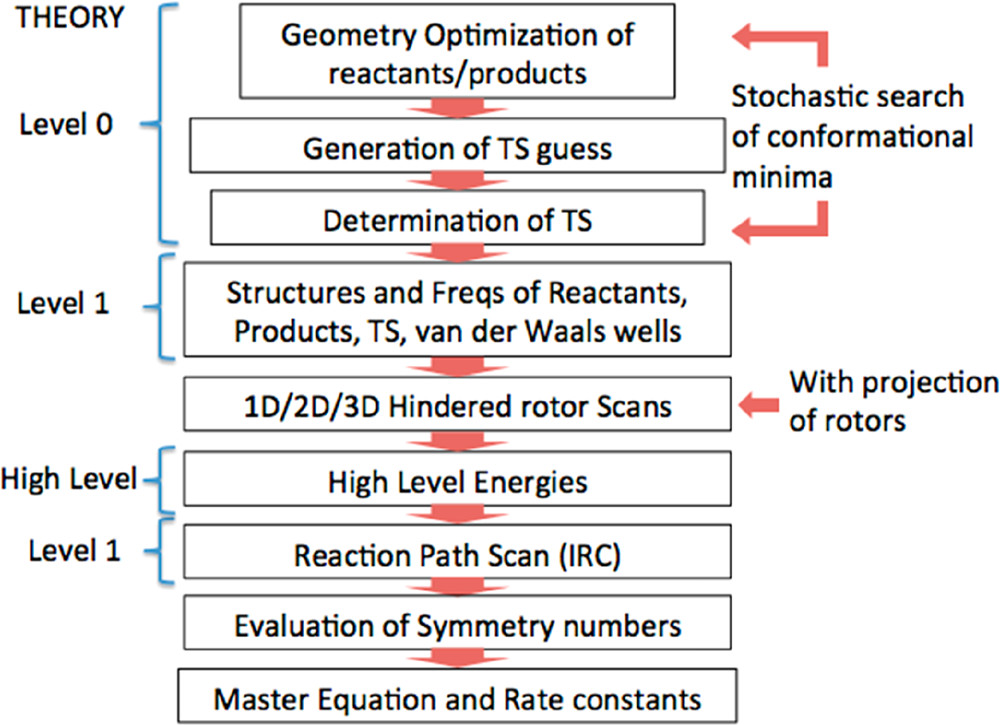
\includegraphics[width=1\textwidth]{estoktp}
    \caption{Program structure of EStokTP.}
    \label{fig:estoktp_structure}
\end{figure}


\begin{figure}
    \centering
    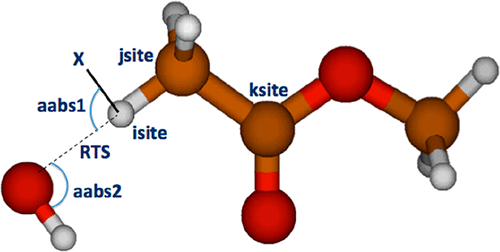
\includegraphics[width=1\textwidth]{estoktp_habstraction}
    \caption{TS geometry constructed for H abstraction in the \ce{OH} + methylacetate reaction. Figure borrowed from \cite{estoktp:2018}}
    \label{fig:estoktp_habstraction}
\end{figure}

Cavollotti and co-workers studied test sets of hydrogen abstraction and addition reactions, and discussed EStokTP's handling of isomerization, beta-scission, barrierless, and multiple well reactions.
Although the methodology for barrierless reactions is promising, this class of reactions would benefit from variable reaction coordinate TST to accurately describe the translational modes within this class of reactions.


%%%%%%%%%%%%%%%%%%%%%%%%%%%%%%%%%%%%%%%%%%%%%%%%%%%%%%%%%%%%%%%%%%%%%%%%%%%%%%%%%%%%
%%%%%%%%%%%%%%%%%%%%%%%%%%%%%%%%%%%%%%%%%%%%%%%%%%%%%%%%%%%%%%%%%%%%%%%%%%%%%%%%%%%%
%%%%%%%%%%%%%%%%%%                                                %%%%%%%%%%%%%%%%%%
%%%%%%%%%%%%%%%%%%                     KinBot                     %%%%%%%%%%%%%%%%%%
%%%%%%%%%%%%%%%%%%                                                %%%%%%%%%%%%%%%%%%
%%%%%%%%%%%%%%%%%%%%%%%%%%%%%%%%%%%%%%%%%%%%%%%%%%%%%%%%%%%%%%%%%%%%%%%%%%%%%%%%%%%%
%%%%%%%%%%%%%%%%%%%%%%%%%%%%%%%%%%%%%%%%%%%%%%%%%%%%%%%%%%%%%%%%%%%%%%%%%%%%%%%%%%%%

\subsection{KinBot (2018)}


KinBot \cite{kinbot:2018, kinbot:2019}, developed by Zador and co-workers at Sandia National Labs, crosses the bridge between reaction mechanism generation, automatic TST calculations, and PES exploration.
Because this review focuses on TST, reference the recent publication by Van de Vijver and Zador for a detailed description of KinBot's PES exploration methods \cite{kinbot:2019}.
KinBot is freely available through the BSD 3-Clause liscense.

To run KinBot, a user would provide a simple input file describing the structure of the species of interest (via SMILES string or Cartesian coordinates), species multiplicity, quantum methods, reaction families of interest, and additional options. 
KinBot first performs a systematic or random conformational search and a geometry optimization of the reactant geometries using the Gaussian quantum chemistry suite.
By default, a systematic conformer search will iterate through all rotatable dihedrals and orientations of cyclic substructures. 
Conformers are then optimized at a L1 level of theory to identify the lowest energy conformer, which is then optimized to calculate frequencies at a L2 level of theory.
If the reactant provided contains many rotatable bonds, a user may specify a maximum number of samples to use during a calculation, and the use of a random sampling mechanism rather than the default.
To ensure the lowest energy conformer is isomorphic to the starting species and TS, KinBot will ensure no bond lengths significantly change, resulting in unwanted rearrangements of atoms.

\begin{figure}
    \centering
    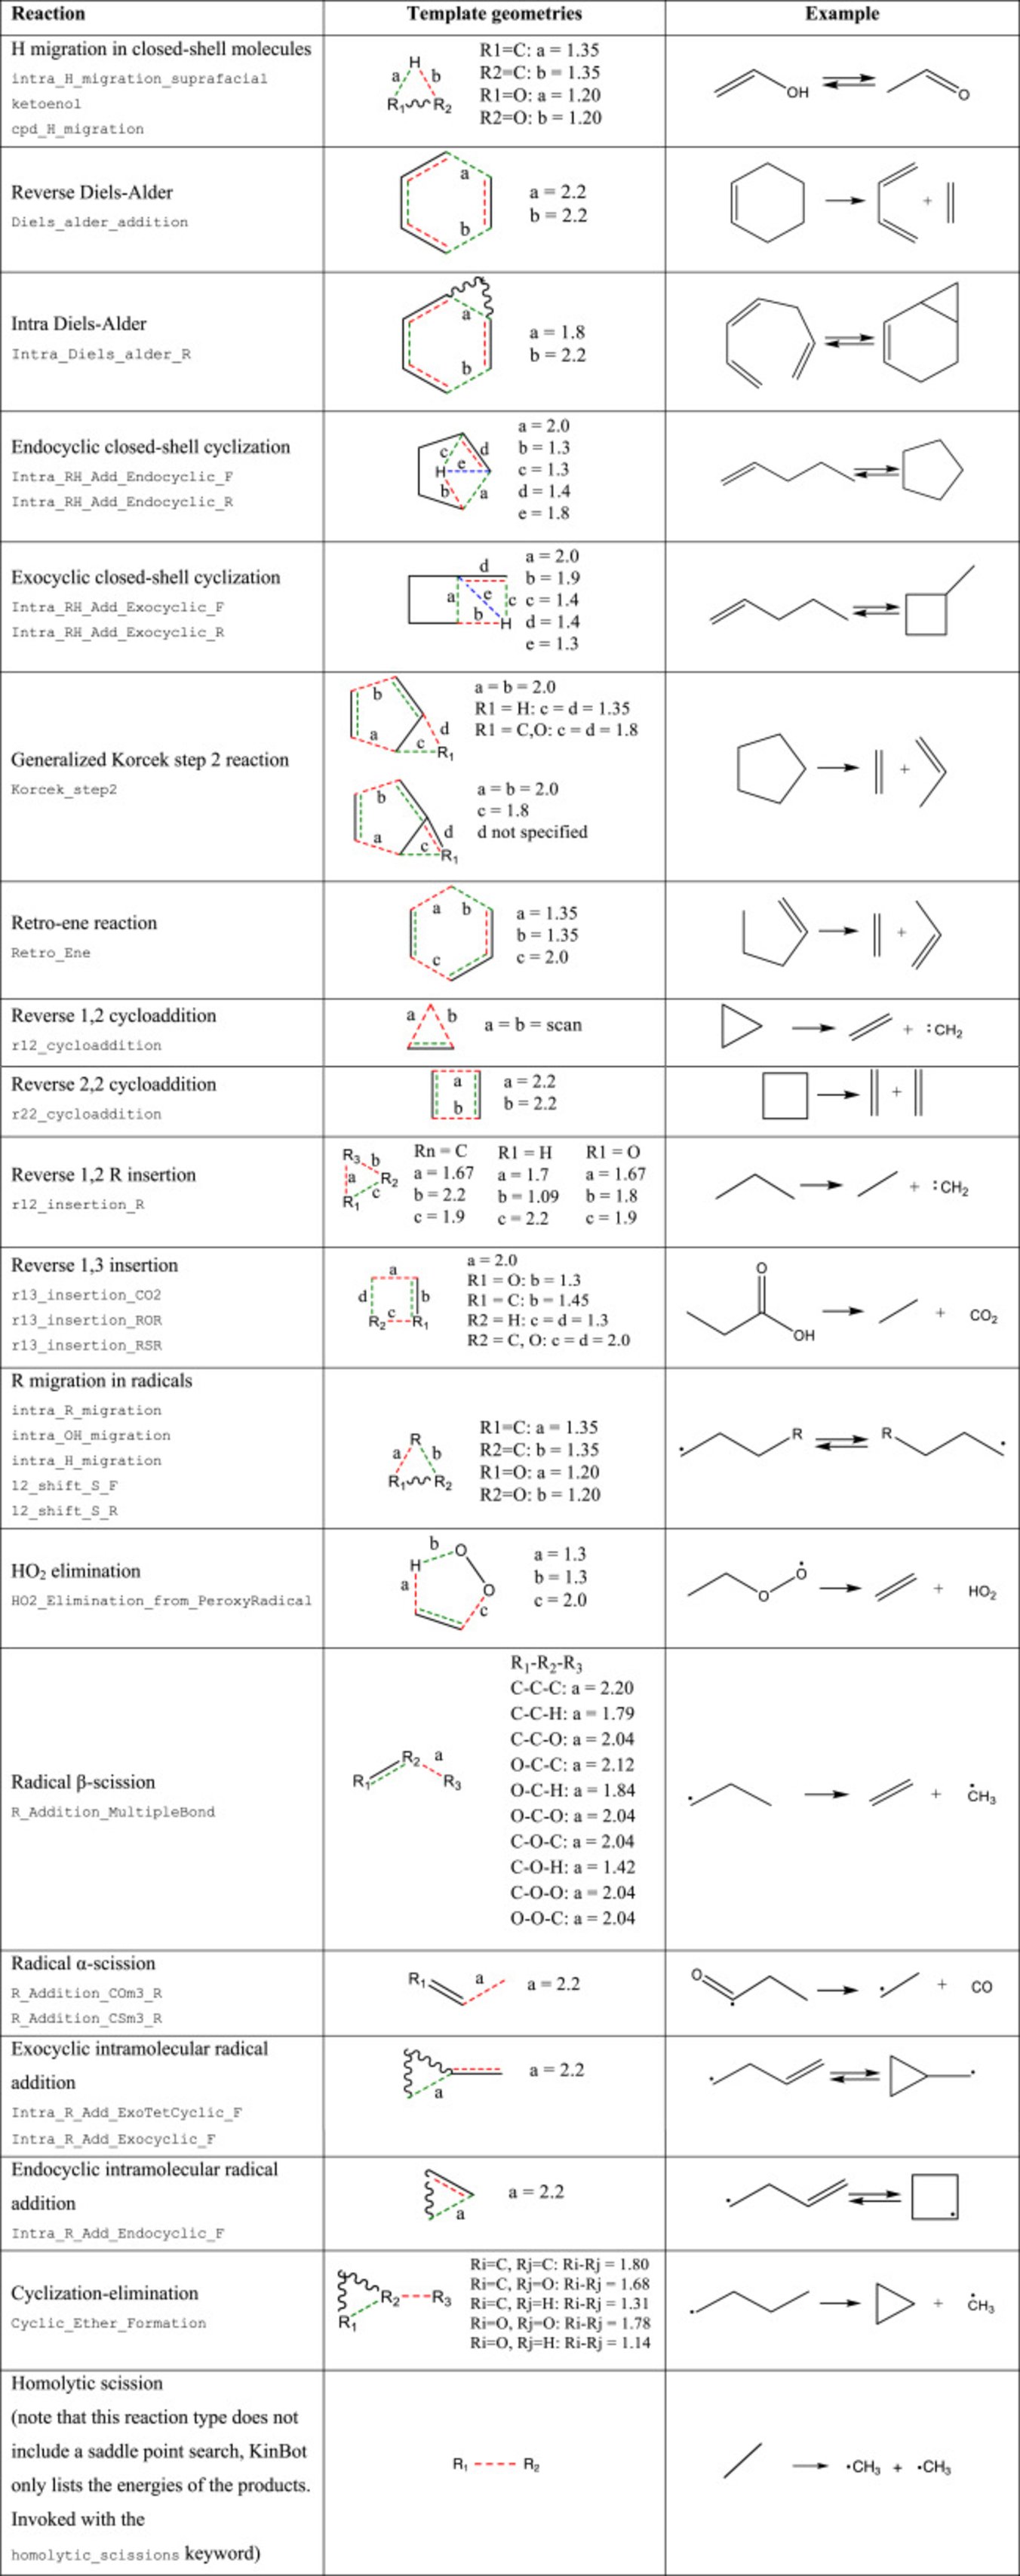
\includegraphics[width=0.5\textwidth]{kinbot_reactions}
    \caption{A table describing all of the reaction families supported by KinBot,  from \cite{kinbot:2019}.}
    \label{fig:kinbot_families}
\end{figure}

KinBot also relies on predefined reaction families, or general reaction templates, when generating mechanisms. 
From a user specified list of reaction families (figure \ref{fig:kinbot_families}), KinBot will then set up a TS guess using either a ``direct'', ``indirect'', or ``scan'' strategy performed at a low level of theory (L0).
Through the direct and indirect methods, a transition state guess is created by performing a series of geometry modifications and constrained optimizations to bring reacting atoms to a specified distance. 
Dihedrals, angles, and bonds of the complex are modified (in that order) and undergo a constrained optimization with modified variable frozen.
If the direct or indirect method results in a poor guess, KinBot will use the scan method, where the TS guess is created by scanning the electronic energies along the active bond and by selecting the maximum energy complex.

Once a TS guess is identified, the geometry is optimized to a first-order saddle point with a L1 level of theory, and if a saddle point is found, the geometry is re-optimized and frequencies are calculated at a L2 level of theory.
TS geometries are validated by IRC calculations and by asserting (1) that resultant reactants matches the input reactants and (2) the product side of the geometry results in a product structure different than the input geometry generated by KinBot (e.g. \ce{A <=> A} isn't the resultant reaction).
For TS and product geometries, conformer analysis is performed identical to the reactants; however, TS geometries require special treatment. 
Given that TSs are undergoing the breaking and forming of bonds, identification of bonds from Cartesian coordinates is not as simple as in stable species.
The TS conformer analysis will identify active bonds comparing reactants and products when creating complexes. 
Cyclic TSs are considered to be rings when performing conformational analysis.

Once reactant, product, and TS geometries are identified, internal rotors are scanned (if requested by the user) at a L2 level of theory.
KinBot systematically scans each rotatable dihedral in \ang{30} increments and performs constrained optimizations, from which potentials are fitted to a Fourier expansion.
%defined by equation \ref{eq:hinderedrotor_kinbot} where $V_{ci}$ and $V_{si}$ are fitted parameters and $\phi$ is the dihedral.
This fitted curve is then used in Master Equation codes to account for hindered rotations.
Additionally, if a lower energy conformer is identified while performing said scans (i.e. if a user does not specify an exhaustive search), the scan is restarted with the new lower energy conformer.

%\begin{equation}
%    V = \Sigma^{6}_{i=1} V_{ci}(1 - \cos(i \cdot \phi)) + \Sigma^{6}_{i=1} V_{si} \sin(i \cdot \phi)
%    \label{eq:hinderedrotor_kinbot}
%\end{equation}

Next, KinBot determines the symmetry number of reactants, products, and TS geometries using a set of rules based on atom, bond, and cycle contributions.
KinBot will first iterate through atoms not present in a ring, will identify the number of neighbors and equivalent neighbors for each atoms, and determine the each atom's contribution to the external symmetry using a tabular method.
Then it will iterate through all bonds and linear structures (\ce{C=C=C}) and, if the terminal atoms on either end of the bond or structure are equivalent, the external symmetry is increased by a factor of two.
In addition, if neighbors of the terminal atoms are equivalent, the external symmetry is increased depending on the equivalence.
Rings are broken at a bond to create a vector based on atom type and indexes, and this vector is ``rolled'' by shifting atom indexes by 1 while maintaining the order and is repeated to create all possible vectors.
This process is also repeated in the reverse direction (e.g. if the first vector created for a 6 member ring has indexes [1, 2, 3, 4, 5, 6] the reverse vector would be [1, 6, 5, 4, 3, 2]).
The reverse vector is also ``rolled'' and all possible vectors are stored.
At this point, the number of vectors that are atom type identical to the initial forward vector are counted and defined as $n$ and the ring contribution to the symmetry is defined as $n+1$. 

Finally, KinBot (at the users request) performs single point energy calculations at a L3 level of theory.
All calculations that performed by KinBot are able to be used in two master equation codes: MESS \cite{MESS:2013} or MESMER \cite{MESMER:2012}, where only minor manual input is required to perform rate estimations.

Van de Vijver and Zador tested the efficacy of KinBot on four different test sets: [1,3]-sigmatropic H-migration reactions, thermal decomposition of gamma-valerolactone, propene and OH, and Aramco Mech up to C4 species.
The authors do not comment on improvement in the article itself, but point to \texttt{kinbot.sandia.gov} and the KinBot manual for descriptions of improvements.


%%%%%%%%%%%%%%%%%%%%%%%%%%%%%%%%%%%%%%%%%%%%%%%%%%%%%%%%%%%%%%%%%%%%%%%%%%%%%%%%%%%%
%%%%%%%%%%%%%%%%%%%%%%%%%%%%%%%%%%%%%%%%%%%%%%%%%%%%%%%%%%%%%%%%%%%%%%%%%%%%%%%%%%%%
%%%%%%%%%%%%%%%%%%%%%%%%%%%%%%%%%%%%%%%%%%%%%%%%%%%%%%%%%%%%%%%%%%%%%%%%%%%%%%%%%%%%

\section{Discussion}
%

This review summarizes existing code bases that can perform automated TST calculations.
%But it is hard to definitively say one code is ``best'' because the definition of ``best'' is subjective and near impossible to define.
Though all of these code bases fall under the umbrella of automated TST calculations, each has features to tackle specific issues well.
AutoTST provides high throughput calculations that perform better than most rate estimations, AutoTS finds TS geometries for almost any reaction family, Genesys provides on the fly calculations with little user input, AARON handles reactions involving transition metals, EStokTP provides high fidelity rate expressions with less user input than traditional TS searches, and KinBot bridges the gap between mechanism generation and automated TST calculations. 
This review has dentified that many code bases contain the following:
\begin{enumerate}
    \item Input method,
    \item A way to generate a TS guess,
    \item A way to arrive at a TS geometry,
    \item Tools to validate a TS geometry,
    \item Conformer analysis,
    \item Consideration of hindered rotors,
    \item Addition of single-point energies,
    \item Calculation of symmetry number,
    \item and a way to determine kinetic parameters.
\end{enumerate}

Each of these categories plus a few more are summarized in table \ref{table:comparison}. 

\newgeometry{top=0.4in, bottom=1in, left=0in, right=0in} 
\begin{table}[h!]
\caption{A table describing the reviewed codes that describes their differences.}
\label{table:comparison}
\begin{center}
\begin{singlespace}
\begin{adjustbox}{angle=90}
\begin{scriptsize}
\begin{tabular}{m{0.45in}||m{0.25in} | m{0.45in} | m{0.8in} | m{0.7in}| m{0.5in}| m{0.5in }|m{0.45in}| m{0.45in}| m{0.5in}| m{0.45in}| m{0.5in}| m{0.5in} | m{0.45in}}
    
    Software & Year Published & Input & Generation of Guesses & Geometry Optimizations & Conformer Analysis & Validation & Hindered Rotors & Zero Point Energies & Symmetry & Kinetics & Supported QM Software & Supported Atoms & Open Source? Licensing? \\
    \hline
    \hline
    AutoTST & 2016 & RMG reaction, reaction family & Identifies key distances based on functional groups in reaction center, embeds at L0. & Series of partial optimizations at L2 & No & IRC Calculation & No & No & Yes, SYMMETRY package in RMG & Yes, Arkane & Gaussian & H, C, O. Partial support for Cl, N, S, Si & Yes, MIT license \\
    \hline
    AutoTS  & 2017 & 3D geometries of reactants and products & IDs active bonds through systematic deletion, Linear regression along reaction coordinates to find energy maximum at L2. Templates previous run reaction to reaction of interest. & QST search using reactants, products, and TS guess at L2 & No & Vetting and Connecting & No & No & No & No & Jaguar & All atom types & No, proprietary license \\
    \hline 
    Genesys & 2018 & Guess of reaction center coordinates, reaction family & Uses key distances to embed with L0 & Low level optimization and Conformer analysis ad L1, Final optimization at L2 & Yes, systematic & Normal mode analysis & Yes, 1D & Yes, L3 calculation & Unspecified & Yes, by hand & Gaussian& H, C, O, S & No, not distributed \\ 
    \hline
    AARON   & 2018 & Reaction template, labeled atoms & Template previous run reaction to reaction of interest & Partial optimizations at L2 & Yes, rule based & ``Step Vetting'' Validation & No & No & No & No & Gaussian & All atom types & Yes, GPL-3.0 license \\ 
    \hline
    EStokTP & 2018 & Guesses of reaction center coordinates, reaction family & Uses provided internal coordinates to construct 3D geometry & Conformer search at L2, series of partial optimizations at L2 theory & Yes, stochastic & IRC Calculation &Yes, 1D, 2D, 3D & Yes, L3 calculation & Yes, MESS package & Yes, AITSTME & Gaussian, MolPro & H, C, O, S, N & Yes, GPL-3.0 license  \\ 
    \hline
    KinBot  & 2019 & SMILES or 3D coordinates of reactant, reaction families of interest & Indirect or direct setting of reaction center, relaxation of reaction shell. Scan along active bonds.  & L0 search for conformer analysis, L2 search for final optimization. & Yes, systematic or random & IRC Calculation & Yes, 1D & No & Yes, graph based approach & Yes, MESS or MESMER & Gaussian & H, C, O, S & Yes, BSD 3-Clause license \\ 
    \hline
   
\end{tabular}
\end{scriptsize}
\end{adjustbox}
\end{singlespace}
\end{center}
\end{table}
\restoregeometry
%In addition, each of these code bases lies somewhere on the plot of fidelity vs throughput. 
%We suggest a qualitative comparison of fidelity vs throughput for previously discussed code bases, rate rule estimations, and parameters determined via experimentation in figure \ref{fig:autokin_comparison}.
Though each of these code bases are effective, there is currently no tool that attains the desired high throughput \textit{and} high fidelity required to calculate kinetic rates for entire reaction mechanisms.
The end goal of automated kinetics should strive for open-source codes that allow users to perform high fidelity TST calculations on reactions involving any atom type and for all reaction families (homo- and heterogeneous).
This software should: require simple inputs to create an educated guess of the TS geometry; perform a through conformational analysis and hindered rotor scans on all reactants, products, and TS geometries; calculate zero point energies; calculate symmetry numbers of complexes accurately; and estimate kinetic parameters while being able to work on a variety of reaction types, atom types, quantum software packages, and high performance computing environments.

AutoTST, AutoTS, AARON, and KinBot allow libraries of previously results to generate TS guesses but AutoTS is able to provide these guesses when no training data exists as well.
Being able to generate TSs with and without training data is highly sought after and should be included in future developments of softwares.
In addition, generalizability is desired -- both AutoTS and AARON support many atom types and AutoTS can perform calculations on almost any reaction family, both of these features should be included in future software.
A detailed conformational analysis is of great importance and the stochastic and systematic methods that exist in AARON, KinBot, Genesys, and EStokTP allow for effective exploration of conformational space.
Hindered rotor scans and zero point energy calculations in KinBot, Genesys, and EStokTP help to more accurately estimate the kinetics of a reaction.
Finally, the determination of symmetry numbers and coupling to a statistical mechanics or master equation solver is necessary to obtain kinetics and is currently present in AutoTST, Genesys, KinBot and EStokTP.

The presence of many code bases is advantageous to perpetuate research through competition, but it can also slow the progress (the reinventing of the wheel may not be entirely necessary in some cases).
A collaborative effort should be made, when possible, to allow codes and their developers to interact and communicate with one another to further develop the field of automated TST.



\section{Acknowledgements}

This material is based upon work supported by the National Science Foundation under Grant No. 1605568.
The authors were partially supported by the U.S. Department of Energy, Office of Science, Basic Energy Sciences, under Award \#0000232253, as part of the Computational Chemical Sciences Program.



\bibliography{refs.bib}
\bibliographystyle{elsarticle-num}


\end{document}
